%Document-Author: Maino Elia
%Document-Date: 2016/05/29
%Document-Description: Documento di Definizione di prodotto del gruppo SWEeneyThreads 

\documentclass[a4paper]{article}
\usepackage[english, italian]{babel}
\usepackage[T1]{fontenc}
\usepackage[utf8]{inputenc}
\usepackage{url}
\usepackage{graphicx}
\usepackage[hidelinks]{hyperref}
\usepackage{booktabs}
\usepackage{eurosym}
\usepackage{tabularx}
\usepackage{pifont}
\usepackage[table]{xcolor}
\usepackage{float}
\usepackage[]{appendix}
\usepackage{ltxtable} 
\usepackage{geometry}
\geometry{margin=1in}
\usepackage{longtable}
\usepackage{multirow}

\graphicspath{{Immagini/DP/}}

\newcolumntype{Y}{>{\centering\arraybackslash}X}
\newcolumntype{s}{>{\hsize=.21\hsize}X}
\newcolumntype{f}{>{\hsize=.37\hsize}X}
\newcolumntype{m}{>{\hsize=.42\hsize}X}
\newcolumntype{t}{>{\hsize=.1\hsize}X}
\newcolumntype{r}{>{\hsize=.3\hsize}X}
\newcolumntype{k}{>{\hsize=.4\hsize}X}

\renewcommand{\abstractname}{Tabella contenuti}

\begin{document}
	
	\begin{titlepage}
		% Defines a new command for the horizontal lines, change thickness here
		\newcommand{\HRule}{\rule{\linewidth}{0.5mm}} 
		\center  
		
		% HEADING SECTION
		\textsc{\LARGE SWEeneyThreads}\\[1.5cm] 
		\textsc{\Large Actorbase}\\[0.5cm] 
		\textsc{\large a NoSQL DB based on the Actor model}\\[0.5cm]
		
		
		% TITLE SECTION
		\HRule \\[0.4cm]
		{ \huge \bfseries Definizione di prodotto}\\[0.4cm] 
		\HRule \\[1.5cm]
		
		% AUTHOR SECTION
		\begin{minipage}{0.4\textwidth}
			\begin{flushleft} \large
				\emph{Redattori:}\\
				Maino Elia \\
			\end{flushleft}
		\end{minipage}
		~
		\begin{minipage}{0.4\textwidth}
			\begin{flushright} \large
				\emph{Approvazione:} \\
                    \dots \\
				\emph{Verifica:} \\
                    \dots \\
				 
			\end{flushright}
		\end{minipage}
		
		%immagine
		\begin{figure}[H]
			\centering
			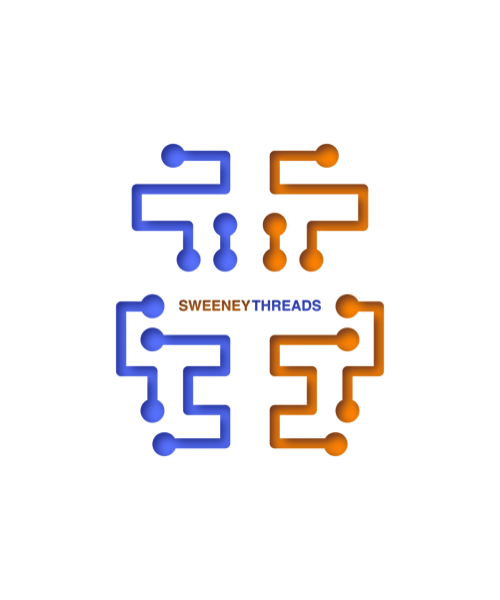
\includegraphics[scale=0.8]{sweeney.png}
		\end{figure}
		\begin{center}
			Versione 0.0.4
		\end{center}
		% Date, change the ->day to a set date if you want to be precise
		{\large \today} \\ [3cm] 
		% Fill the rest of the page with whitespace
		\vfill  
	\end{titlepage}
	
	
	\tableofcontents
	
	\newpage 
	\section*{Diario delle modifiche}
		\LTXtable{\textwidth}{Tabelle/tabelle_diario_modifiche/tabella_definizione.tex}

	\newpage \section{Introduzione}
	\subsection{Scopo del documento}
		Il documento illustra la progettazione di dettaglio del software \emph{Actorbase}.
		Le decisioni architetturali definite nel documento di \emph{Specifica Tecnica} saranno sviluppate ad un livello di dettaglio superiore, tale da fornire uno strumento adeguato a guidare e supportare l'attività di programmazione del gruppo.
	\subsection{Scopo del prodotto}
		Il progetto consiste nella realizzazione di un Database NoSQL key-value basato sul modello ad 
		Attori con l'obiettivo di fornire una tecnologia adatta allo sviluppo di moderne 
		applicazioni che richiedono brevissimi tempi di risposta e che elaborano enormi quantità 
		di dati. Lo sviluppo porterà al rilascio del software sotto licenza MIT.
	\subsection{Glossario}
		Al fine di evitare ambiguità di linguaggio e di massimizzare la comprensione dei documenti, il 
      gruppo ha steso un documento interno che è il \emph{Glossario v2.0.0}. In esso saranno definiti, in modo
      chiaro e conciso i termini che possono causare ambiguità o incomprensione del testo.
	\subsection{Riferimenti}
		\begin{itemize}
			\item \textbf{Slide dell'insegnamento Ingegneria del software mod.A:} \\
			\url{http://www.math.unipd.it/~tullio/IS-1/2015/Dispense/E02.pdf}
			\item \textbf{Scala:} \\
			\url{http://www.scala-lang.org/}
			\item \textbf{Java:} \\
			\url{http://www.java.com/}
			\item \textbf{Akka:} \\
			\url{http://akka.io/}
			\item \textbf{IntelliJ:} \\
			\url{http://www.jetbrains.com/idea/}
		\end{itemize}
	\textbf{Normativi}
		\begin{itemize}
			\item \textbf{Norme di progetto:} \emph{Norme di progetto v2.0.0}
			\item \textbf{Capitolato d'appalto Actorbase (C1):} \\ 
			\url{http://www.math.unipd.it/~tullio/IS-1/2015/Progetto/C1p.pdf}
		\end{itemize}
		
	\newpage	
	
	\section{Standard di progetto}
		Di seguito si riportano gli standard di progettazione e documentazione a cui i membri del gruppo dovranno attenersi durante l'attività di progettazione di dettaglio e programmazione.
	\subsection{Standard di progettazione}
		Gli standard di progettazione architetturale sono definiti nei documenti di \emph{Specifica Tecnica 3.0.0} e \emph{Norme di Progetto 3.0.0, sez 2.2.6}.  
	\subsection{Standard di codifica}
		Gli standard di codifica sono definiti nel documento \emph{Norme di Progetto 3.0.0, sez 2.2.11}.
	\subsection{Standard di documentazione del codice}
		Gli standard relativi alla documentazione del codice prodotto sono definiti nel documento \emph{Norme di progetto 3.0.0, sez 2.2.11}.
	\subsection{Strumenti di lavoro}
		Gli strumenti di lavoro da utilizzare sono definiti nel documento \emph{Norme di Progetto 3.0.0}.
		
	\newpage
	
	\section{Specifica componenti}
		In tale sezione verranno descritti il più dettagliatamente possibile i componenti architetturali definiti nel documento \emph{Specifica Tecnica}.
		
	\subsection{Actorbase}
		\begin{figure}[H]
			\centering
			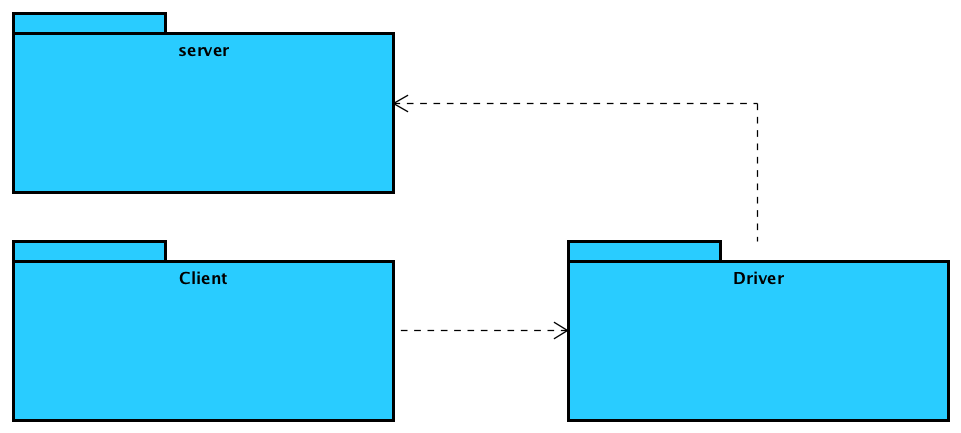
\includegraphics[width=\textwidth]{generalLevel.png}
			\caption{Actorbase architettura generale}
		\end{figure}
		L'architettura generale di \emph{Actorbase} è formata da tre componenti: Server, Client e Driver. 
		Il Client utilizza metodi e oggetti forniti dal Driver per comunicare con il Server.
		
	\subsection{Actorbase.server}
		\begin{figure}[H]
			\centering
			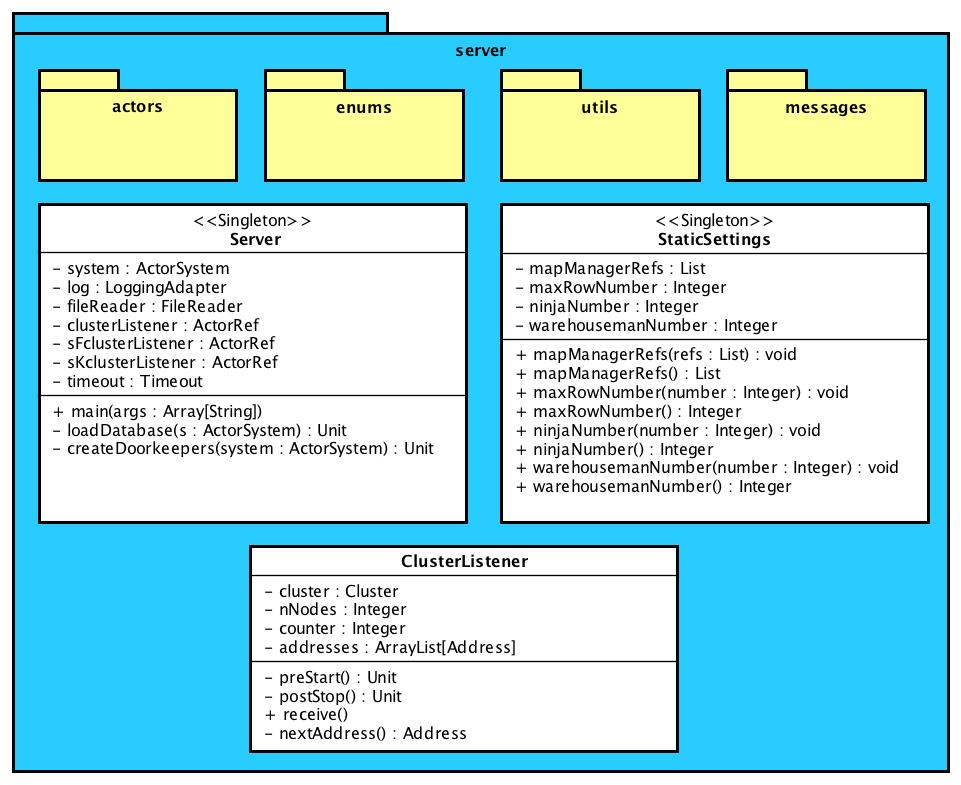
\includegraphics[scale=0.5]{Server/serverLevel.jpg}
			\caption{Componente Actorbase.server}
		\end{figure}
		La componente server di \emph{Actorbase} è il nucleo dell'applicativo, è composta dai packages: utils, messages, actors ed enums e dalla classe Server.
		
	\subsection{Actorbase.server.Server (Object)}
		\begin{figure}[H]
			\centering
			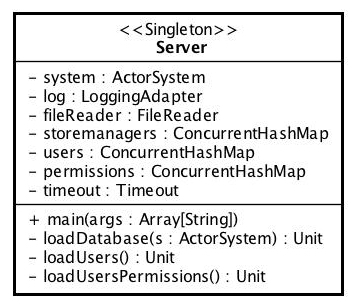
\includegraphics[scale=0.5]{Server/serverClass.jpg}
			\caption{Classe Actorbase.server.Server}
		\end{figure}
		\textbf{Descrizione}
			\\ \\
			Classe principale della parte Server del programma. \'E di fatto l'entry point dello stesso, gestisce la configurazione iniziale e avvia il sistema. Utilizza il design pattern Singleton (Object).
			\\ \\
		\textbf{Utilizzo}
			\\ \\
			Classe che fornisce un punto di accesso al programma, la sua esecuzione avvia il server sulla macchina in cui viene lanciata (contiene il metodo \texttt{main} per la componente server di \emph{Actorbase}).
			\\ \\
		\textbf{Classi ereditate}
			\\ \\
			Nessuna.
			\\ \\
		\textbf{Ereditata da}
			\\ \\
			Nessuna.
			\\ \\
		\textbf{Attributi}
			\begin{itemize}
				\item \texttt{val system: ActorSystem } - Istanza di ActorSystem di Akka.
				\item \texttt{var log: LoggingAdapter } - Permette di ottenere un log per l'ActorSystem.
				\item \texttt{implicit val timeout: Timeout } - Timeout di connessione.
				\item \texttt{var clusterListener: ActorRef} - Cluster
				\item \texttt{var sFclusterListener: ActorRef} - Cluster
				\item \texttt{var sKclusterListener: ActorRef} - Cluster
			\end{itemize}
			\textbf{Metodo: }\texttt{main(args: Array[String]}
			\\ \\
			Metodo main che permette di avviare l'applicativo lato server. Si occupa di impostare i valori dei campi dati e di invocare gli altri metodi di configurazione presenti nella classe.
			\\ \\
			Lista parametri del metodo:
			\begin{itemize}
				\item \texttt{args: Array[String] } - Parametro standard del metodo main di \emph{Scala}.
			\end{itemize}
			\textbf{Metodo: }\texttt{private def loadDatabases(system: ActorSystem): Unit}
			\\ \\
			Il metodo carica i database da disco.
			\\ \\
			Lista parametri del metodo:
			\begin{itemize}
				\item \texttt{system: ActorSystem } - ActorSystem da utilizzare per accedere agli attori necessari.
			\end{itemize}
			\textbf{Metodo: }\texttt{private def createDoorkeepers(system: ActorSystem): Unit}
			\\ \\
			Legge le impostazioni di configurazione degli attori \texttt{Doorkeeper} e si occupa della conseguente creazione degli attori stessi.
			\\ \\
			Lista parametri del metodo:
			\begin{itemize}
				\item \texttt{system: ActorSystem } - ActorSystem da utilizzare per accedere agli attori necessari.
			\end{itemize}
			
		\subsection{Actorbase.server.StaticSettings (Object)}
		Immagine UML.
		\\ \\
		\textbf{Descrizione}
			\\ \\
			Classe statica che permette di accedere a dei dati (impostazioni) globali.
			\\ \\
		\textbf{Utilizzo}
			\\ \\
			La classe definisce i valori di alcune proprietà che devono essere utilizzati da diversi componenti del sistema, evitando il passaggio di tali dati tra le componenti. Alcuni dei dati che la classe contiene devono essere:
			\begin{itemize}
				\item Riferimento agli attori \texttt{MapManager} presenti
				\item Numero massimo di righe per \texttt{Storemanager} (di tipo \texttt{Storekeeper})
				\item Numero di attori \texttt{Ninja}
				\item Numero di attori \texttt{Warehouseman}
			\end{itemize}
		\textbf{Classi ereditate}
			\\ \\
			Nessuna.
			\\ \\
		\textbf{Ereditata da}
			\\ \\
			Nessuna.
			\\ \\
		\textbf{Attributi}
			\begin{itemize}
				\item \texttt{var mapManagerRefs: ConcurrentHashMap[String, ActorRef]} - Riferimento ai \texttt{MapManger}.
				\item \texttt{var maxRowNumber: Integer} - Numero massimo di righe.
				\item \texttt{var ninjaNumber: Integer } - Numero di \texttt{Ninja}.
				\item \texttt{var warehousemanNumber: Integer} - Numero di \texttt{Warehousean}.
			\end{itemize}
			
		\subsection{Actorbase.server.ClusterListener }
		Immagine UML.
		\\ \\
		\textbf{Descrizione}
			\\ \\
			La classe rappresenta l'attore responsabile di mantenere gli indirizzi dei nodi segnati come \emph{UP} nel cluster. Deve esserci un attore \texttt{ClusterListener} in ogni nodo del cluster. L'attore inoltre implementa una strategia Round Robin per selezionare un indirizzo dalla sua lista di nodi.
			\\ \\
		\textbf{Utilizzo}
			\\ \\
			Questo attore viene utilizzato per gestire le funzionalità del Cluster.
			\\ \\
		\textbf{Classi ereditate}
			\begin{itemize}
				\item \texttt{akka.actor.Actor}
				\item \texttt{akka.actor.ActorLogging}
			\end{itemize}
		\textbf{Ereditata da}
			\\ \\
			Nessuna.
			\\ \\
		\textbf{Attributi}
			\begin{itemize}
				\item \texttt{private val cluster: Cluster} - L'istanza del cluster.
				\item \texttt{private var nNodes: Integer } - Numero di nodi \emph{UP} nel cluster (inizialmente 0).
				\item \texttt{var counter: Integer} - Contatore delle richieste (inizialmente a 0). Deve essere incrementato prima di ogni operazione.
				\item \texttt{var addresses: ArrayList[Address]} - Lista degli indirizzi dei nodi del cluster.
			\end{itemize}
			\textbf{Metodo: }\texttt{override def preStart(): Unit}
			\\ \\
			Override del metodo \texttt{preStart()} definito in \texttt{akka.actor.Actor}. Alla creazione dell'attore esso si sottoscrive al cluster e aggiunge l'indirizzo del suo nodo alla lista.
			\\ \\
			Lista parametri del metodo:
			\\ \\
			Nessuno.
			\\ \\
			\textbf{Metodo: }\texttt{override def postStop(): Unit}
			\\ \\
			Override del metodo \texttt{postStop()} definito in \texttt{akka.actor.Actor}. Allo stop l'attore deve rimuoversi dal cluster.
			\\ \\
			Lista parametri del metodo:
			\\ \\
			Nessuno.
			\\ \\
			\textbf{Metodo: }\texttt{def receive}
			\\ \\
			Metodo di ricezione dei messaggi dell'attore, il metodo riceve messaggi dal cluster e il messaggio (stringa) \texttt{"next"} (richiesta di rotazione Round Robin). I messaggi ricevuti dal cluster vengono gestiti in modo da mantenere la lista dei nodi aggiornata. Il metodo gestisce i seguenti messaggi:
			\begin{itemize}
				\item \texttt{MemberUp}
				\item \texttt{UnreachableMember}
				\item \texttt{MemberRemoved}
			\end{itemize}
			Lista parametri del metodo:
			\\ \\
			Nessuno.
			\\ \\
		\textbf{Metodo: }\texttt{def nextAddress(): Address}
			\\ \\
			Metodo che implementa la strategia Round Robin per selezionare un indirizzo.
			\\ \\
			Lista parametri del metodo:
			\\ \\
			Nessuno.
			
	\subsection{Actorbase.server.utils}
		\begin{figure}[H]
			\centering
			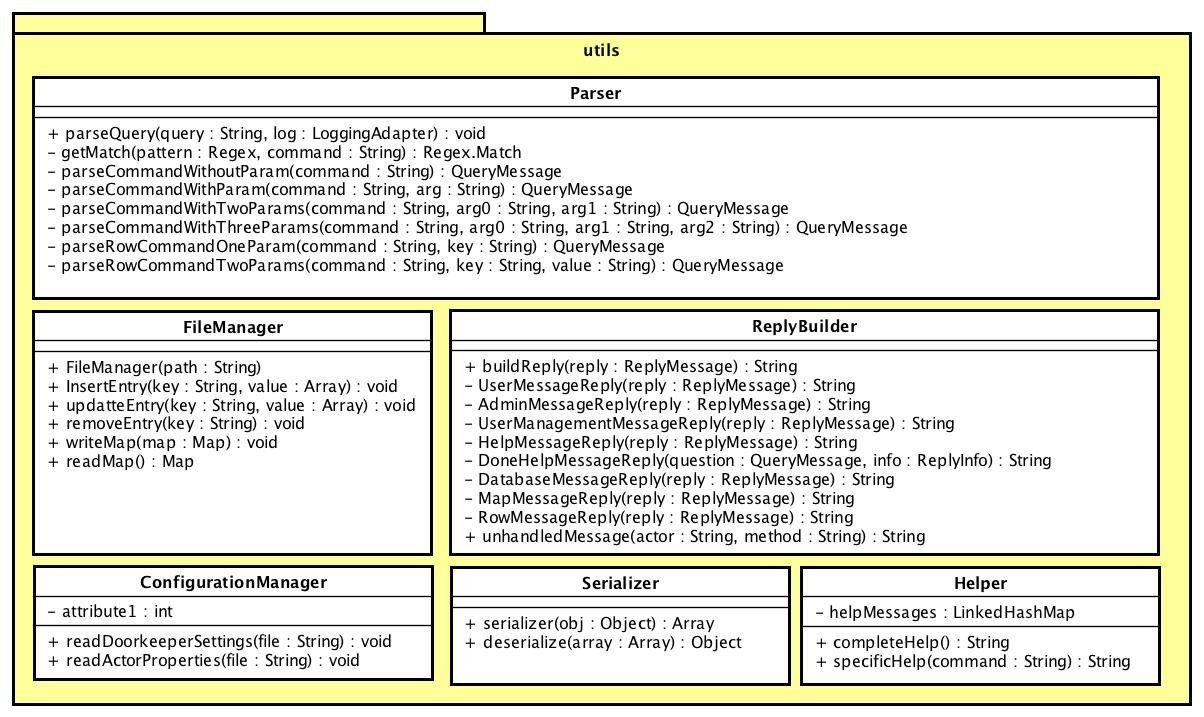
\includegraphics[width=\textwidth]{Server/utilsLevel.jpg}
			\caption{Componente Actorbase.server.utils}
		\end{figure}
		Package contenente le classi che effettuano operazioni varie a supporto delle varie componenti del server, e degli attori nello specifico.
		
			
	\subsection{Actorbase.server.utils.Parser}
		Immagine UML.
		\\ \\
		\textbf{Descrizione}
			\\ \\
			La classe \texttt{Parser} definisce i metodi per trasformare stringhe in messaggi \texttt{QueryMessage} utilizzabili dagli attori del sistema.
			\\ \\
		\textbf{Utilizzo}
			\\ \\
			Viene utilizzata da attori di tipo \texttt{Usermanager} per trasformare le richieste client in messaggi inviabili agli attori.
			\\ \\
		\textbf{Classi ereditate}
			\\ \\
			Nessuna.
			\\ \\
		\textbf{Ereditata da}
			\\ \\
			Nessuno.
			\\ \\
		\textbf{Attributi}
			\\ \\ 
			Nessuno.
			\\ \\
			\textbf{Costruttore: }\texttt{Parser()}
			\\ \\
			Costruttore senza parametri.
			\\ \\
			Lista parametri del metodo:
			\\ \\
			Nessuno.
			\\ \\
			\textbf{Metodo: }\texttt{parseQuery(query: String) : QueryMessage}
			\\ \\
			Effettua il parsing della stringa in base al numero di parametri che la compongono (utilizzando i metodi per il parsing a seconda dei parametri) e genera un \texttt{QueryMessage} che viene ritornato.
			\\ \\
			Lista parametri del metodo:
			\begin{itemize}
				\item \texttt{query: String } - Stringa da convertire in messaggio.
			\end{itemize}
			\textbf{Metodo: }\texttt{getMatch(pattern:Regex, command:String): Regex.Match}
			\\ \\
			Effettua il match dell'espressione regolare sulla stringa passata e ritorna il risultato.
			\\ \\
			Lista parametri del metodo:
			\begin{itemize}
				\item \texttt{pattern: Regex } - Pattern da utilizzare per il match.
				\item \texttt{command: String} - La stringa su cui effettuare il match.
			\end{itemize}
			\textbf{Metodo: }\texttt{parseCommandWithoutParam(command: String): QueryMessage}
			\\ \\
			Effettua il parsing di un comando senza parametri e ritorna il corrispondente \texttt{QueryMessage}.
			\\ \\
			Lista parametri del metodo:
			\begin{itemize}
				\item \texttt{command: String} - La stringa rappresentante il comando.
			\end{itemize}
			\textbf{Metodo: }\texttt{parseCommandWithParam(command: String, arg: String): QueryMessage}
			\\ \\
			Effettua il parsing di un comando con un parametro e ritorna il corrispondente \texttt{QueryMessage}.
			\\ \\
			Lista parametri del metodo:
			\begin{itemize}
				\item \texttt{command: String} - La stringa rappresentante il comando.
				\item \texttt{arg: String} - La stringa rappresentante il parametro.
			\end{itemize}
			\textbf{Metodo: }\texttt{parseCommandWithTwoParams(command:String, arg1: String, arg2: String):QueryMessage}
			\\ \\
			Effettua il parsing di un comando con due parametri e ritorna il corrispondente \texttt{QueryMessage}.
			\\ \\
			Lista parametri del metodo:
			\begin{itemize}
				\item \texttt{command: String} - La stringa rappresentante il comando.
				\item \texttt{arg1: String} - La stringa rappresentante il primo parametro.
				\item \texttt{arg2: String} - La stringa rappresentante il secondo parametro.
			\end{itemize}
			\textbf{Metodo: }\texttt{parseCommandWithThreeParams(command:String, arg1: String, arg2: String, arg3: String):QueryMessage}
			\\ \\
			Effettua il parsing di un comando con tre parametri e ritorna il corrispondente \texttt{QueryMessage}.
			\\ \\
			Lista parametri del metodo:
			\begin{itemize}
				\item \texttt{command: String} - La stringa rappresentante il comando.
				\item \texttt{arg1: String} - La stringa rappresentante il primo parametro.
				\item \texttt{arg2: String} - La stringa rappresentante il secondo parametro.
				\item \texttt{arg3: String} - La stringa rappresentante il terzo parametro.
			\end{itemize}
			\textbf{Metodo: }\texttt{parseRowCommandOneParam(command: String, key: String): QueryMessage}
			\\ \\
			Effettua il parsing di un comando al livello di item con un parametro (la chiave) e ritorna il corrispondente \texttt{QueryMessage}.
			\\ \\
			Lista parametri del metodo:
			\begin{itemize}
				\item \texttt{command: String} - La stringa rappresentante il comando a livello di item.
				\item \texttt{key: String} - La stringa rappresentante la chiave.
			\end{itemize}
			\textbf{Metodo: }\texttt{parseRowCommandTwoParams(command: String, key: String, value: String): QueryMessage}
			\\ \\
			Effettua il parsing di un comando al livello di item con due parametri (la chiave e il valore) e ritorna il corrispondente \texttt{QueryMessage}.
			\\ \\
			Lista parametri del metodo:
			\begin{itemize}
				\item \texttt{command: String} - La stringa rappresentante il comando a livello di item.
				\item \texttt{key: String} - La stringa rappresentante la chiave.
				\item \texttt{value: String} - La stringa rappresentante il valore.
			\end{itemize}
			
			
	\subsection{Actorbase.server.utils.Helper}
		Immagine UML.
		\\ \\
		\textbf{Descrizione}
			\\ \\
			Classe che fornisce i metodi per ottenere una descrizione dei comandi di \emph{Actorbase}.
			\\ \\
		\textbf{Utilizzo}
			\\ \\
			Viene utilizzata per soddisfare una richiesta di \texttt{help} da parte di un utente.
			\\ \\
		\textbf{Classi ereditate}
			\\ \\
			Nessuna.
			\\ \\
		\textbf{Ereditata da}
			\\ \\
			Nessuno.
			\\ \\
		\textbf{Attributi}
			\begin{itemize}
				\item \texttt{helpMessages: LinkedHashMap[String, String] } - Mappa contenente i comandi come chiavi e le descrizioni degli stessi come valori.
			\end{itemize}
		\textbf{Metodo: }\texttt{completeHelp(): String}
			\\ \\
			Il metodo costruisce una stringa contenente l'aiuto completo, basandosi sugli elementi della mappa \texttt{helpMessages}.
			\\ \\
			Lista parametri del metodo:
			\\ \\
			Nessuno.
			\\ \\
		\textbf{Metodo: }\texttt{specificHelp(command: String): String}
			\\ \\
			Il metodo costruisce una stringa contenente l'aiuto per un comando specifico, basandosi sugli elementi della mappa \texttt{helpMessages}.
			\\ \\
			Lista parametri del metodo:
			\begin{itemize}
				\item \texttt{command: String } - Stringa rappresentante il comando per cui si vuole generare il messaggio di aiuto.
			\end{itemize}
			
	\subsection{Actorbase.server.utils.ConfigurationManager}
		Immagine UML.
		\\ \\
		\textbf{Descrizione}
			\\ \\
			Classe che fornisce i metodi di lettura e scrittura dei file di configurazione del server.
			\\ \\
		\textbf{Utilizzo}
			\\ \\
			Viene utilizzata per leggere le impostazioni del server dai file di configurazione all'avvio di esso. Inoltre viene utilizzata per scrivere modifiche alle configurazioni.
			\\ \\
		\textbf{Classi ereditate}
			\\ \\
			Nessuna.
			\\ \\
		\textbf{Ereditata da}
			\\ \\
			Nessuno.
			\\ \\
		\textbf{Attributi}
			\\ \\
			Nessuno.
			\\ \\
		\textbf{Metodo: }\texttt{readDoorkeepersSettings(fileName: String): util.HashMap[String, Integer]}
			\\ \\
			Il metodo legge dal file di configurazione gli indirizzi e le porte che attori di tipo \texttt{Doorkeeper} dovranno utilizzare per gestire le connessioni. Tali informazioni vengono ritornate con una mappa in cui le chiavi sono gli indirizzi e i valori sono le porte.
			\\ \\
			Lista parametri del metodo:
			\begin{itemize}
				\item \texttt{fileName: String} - Nome del file che contiene la configurazione dei \texttt{Doorkeeper}.
			\end{itemize}
		\textbf{Metodo: }\texttt{readActorsProperties(fileName: String): util.HashMap[ActorProperties, Integer]}
			\\ \\
			Il metodo legge dal file di configurazione le proprietà relative agli attori (come ad esempio il numero massimo di attori di tipo \texttt{Ninja}). Tali informazioni vengono ritornate con una mappa in cui le chiavi sono i nomi delle proprietà e i valori sono i valori di tali proprietà.
			\\ \\
			Lista parametri del metodo:
			\begin{itemize}
				\item \texttt{fileName: String} - Nome del file che contiene la configurazione degli attori.
			\end{itemize}
			
	\subsection{Actorbase.server.utils.ReplyBuilder}
		Immagine UML.
		\\ \\
		\textbf{Descrizione}
			\\ \\
			Classe che fornisce i metodi di creazione delle stringhe da mandare in risposta a richieste client.
			\\ \\
		\textbf{Utilizzo}
			\\ \\
			Viene utilizzata per costruire delle risposte in formato stringa a partire da messaggi. Tali risposte possono così essere inviate ad un client.
			\\ \\
		\textbf{Classi ereditate}
			\\ \\
			Nessuna.
			\\ \\
		\textbf{Ereditata da}
			\\ \\
			Nessuno.
			\\ \\
		\textbf{Attributi}
			\\ \\
			Nessuno.
			\\ \\
		\textbf{Metodo: }\texttt{buildReply(reply: ReplyMessage): String}
			\\ \\
			Il metodo permette di costruire una stringa a partire da un \texttt{ReplyMessage}. In particolare questo metodo si occupa di stabilire se il messaggio è di tipo amministratore o utente e delegare di conseguenza l'elaborazione al metodo più appropriato.
			Gestisce i seguenti messaggi:
			\begin{itemize}
				\item \texttt{UserMessage}
				\item \texttt{AdminMessage}
			\end{itemize}
			Lista parametri del metodo:
			\begin{itemize}
				\item \texttt{reply: ReplyMessage} - Il messaggio da cui ricavare la stringa.
			\end{itemize}
		\textbf{Metodo: }\texttt{UserMessageReply(reply: ReplyMessage): String}
			\\ \\
			Il metodo permette di costruire una stringa a partire da un \texttt{ReplyMessage}. In particolare questo metodo si occupa di stabilire che tipo di \texttt{UserMessage} si sia ricevuto.
			Gestisce i seguenti messaggi:
			\begin{itemize}
				\item \texttt{HelpMessage}
				\item \texttt{DatabaseMessage}
				\item \texttt{MapMessage}
				\item \texttt{RowMessage}
			\end{itemize}
			Lista parametri del metodo:
			\begin{itemize}
				\item \texttt{reply: ReplyMessage} - Il messaggio da cui ricavare la stringa.
			\end{itemize}
		\textbf{Metodo: }\texttt{AdminMessageReply(reply: ReplyMessage): String}
			\\ \\
			Il metodo permette di costruire una stringa a partire da un \texttt{ReplyMessage}. In particolare questo metodo si occupa di stabilire che tipo di \texttt{AdminMessage} si sia ricevuto.
			Gestisce i seguenti messaggi:
			\begin{itemize}
				\item \texttt{UsersManagementMessage}
				\item \texttt{PermissionsManagementMessage}
			\end{itemize}
			Lista parametri del metodo:
			\begin{itemize}
				\item \texttt{reply: ReplyMessage} - Il messaggio da cui ricavare la stringa.
			\end{itemize}
		\textbf{Metodo: }\texttt{UserManagementMessageReply(reply: ReplyMessage): String}
			\\ \\
			Il metodo permette di costruire una stringa a partire da un \texttt{ReplyMessage}. In particolare questo metodo si occupa di gestire messaggi di tipo \texttt{UsersManagementMessage}.
			Gestisce i seguenti messaggi:
			\begin{itemize}
				\item \texttt{ListUserMessage}
				\item \texttt{AddUserMessage}
				\item \texttt{RemoveUserMessage}
			\end{itemize}
			Lista parametri del metodo:
			\begin{itemize}
				\item \texttt{reply: ReplyMessage} - Il messaggio da cui ricavare la stringa.
			\end{itemize}
		\textbf{Metodo: }\texttt{PermissionsManagementMessageReply(reply: ReplyMessage): String}
			\\ \\
			Il metodo permette di costruire una stringa a partire da un \texttt{ReplyMessage}. In particolare questo metodo si occupa di gestire messaggi di tipo \texttt{PermissionManagementMessage}.
			Gestisce i seguenti messaggi:
			\begin{itemize}
				\item \texttt{ListPermissionMessage}
				\item \texttt{AddPermissionMessage}
				\item \texttt{RemovePermissionMessage}
			\end{itemize}
			Lista parametri del metodo:
			\begin{itemize}
				\item \texttt{reply: ReplyMessage} - Il messaggio da cui ricavare la stringa.
			\end{itemize}
		\textbf{Metodo: }\texttt{HelpMessageReply(reply: ReplyMessage): String}
			\\ \\
			Il metodo permette di costruire una stringa a partire da un \texttt{ReplyMessage}. In particolare questo metodo si occupa di gestire messaggi di tipo \texttt{HelpMessage} invocando gli opportuni metodi.
			Gestisce i seguenti messaggi:
			\begin{itemize}
				\item \texttt{HelpMessage}
			\end{itemize}
			Lista parametri del metodo:
			\begin{itemize}
				\item \texttt{reply: ReplyMessage} - Il messaggio da cui ricavare la stringa.
			\end{itemize}
		\textbf{Metodo: }\texttt{DoneHelpMessageReply(question: QueryMessage, info: ReplyInfo): String}
			\\ \\
			Il metodo permette di costruire una stringa a partire da un \texttt{ReplyMessage}. In particolare questo metodo si occupa di gestire messaggi di tipo \texttt{HelpMessage} maggiormente nel dettaglio.
			Gestisce i seguenti messaggi:
			\begin{itemize}
				\item \texttt{CompleteHelpMessage}
				\item \texttt{SpecificHelpMessage}
			\end{itemize}
			Lista parametri del metodo:
			\begin{itemize}
				\item \texttt{reply: ReplyMessage} - Il messaggio da cui ricavare la stringa.
			\end{itemize}
		\textbf{Metodo: }\texttt{DatabaseMessageReply(reply: ReplyMessage): String}
			\\ \\
			Il metodo permette di costruire una stringa a partire da un \texttt{ReplyMessage}. In particolare questo metodo si occupa di gestire messaggi di tipo \texttt{DatabaseMessage}.
			Gestisce i seguenti messaggi:
			\begin{itemize}
				\item \texttt{ListDatabaseMessage}
				\item \texttt{SelectDatabaseMessage}
				\item \texttt{CreateDatabaseMessage}
				\item \texttt{DeleteDatabaseMessage}
			\end{itemize}
			Lista parametri del metodo:
			\begin{itemize}
				\item \texttt{reply: ReplyMessage} - Il messaggio da cui ricavare la stringa.
			\end{itemize}
		\textbf{Metodo: }\texttt{MapMessageReply(reply: ReplyMessage): String}
			\\ \\
			Il metodo permette di costruire una stringa a partire da un \texttt{ReplyMessage}. In particolare questo metodo si occupa di gestire messaggi di tipo \texttt{MapMessage}.
			Gestisce i seguenti messaggi:
			\begin{itemize}
				\item \texttt{ListMapMessage}
				\item \texttt{SelectMapMessage}
				\item \texttt{CreateMapMessage}
				\item \texttt{DeleteMapMessage}
			\end{itemize}
			Lista parametri del metodo:
			\begin{itemize}
				\item \texttt{reply: ReplyMessage} - Il messaggio da cui ricavare la stringa.
			\end{itemize}
		\textbf{Metodo: }\texttt{RowMessageReply(reply: ReplyMessage): String}
			\\ \\
			Il metodo permette di costruire una stringa a partire da un \texttt{ReplyMessage}. In particolare questo metodo si occupa di gestire messaggi di tipo \texttt{RowMessage}.
			Gestisce i seguenti messaggi:
			\begin{itemize}
				\item \texttt{ListKeysMessage}
				\item \texttt{FindRowMessage}
				\item \texttt{InsertRowMessage}
				\item \texttt{UpdateRowMessage}
				\item \texttt{RemoveRowMessage}
			\end{itemize}
			Lista parametri del metodo:
			\begin{itemize}
				\item \texttt{reply: ReplyMessage} - Il messaggio da cui ricavare la stringa.
			\end{itemize}
		\textbf{Metodo: }\texttt{unhandledMessage(actor: String, method: String): String}
			\\ \\
			Il metodo permette di costruire una stringa per i messaggi che non sono stati gestiti.
			Lista parametri del metodo:
			\begin{itemize}
				\item \texttt{actor: String} - Il percorso dell'attore che non ha gestito il messaggio
				\item \texttt{method: String} - Il nome del metodo in cui non è stato gestito il messaggio
			\end{itemize}
			
	\subsection{Actorbase.server.utils.Serializer}
		Immagine UML.
		\\ \\
		\textbf{Descrizione}
			\\ \\
			Classe che gestisce la serializzazione e la deserializzazione di oggetti.
			\\ \\
		\textbf{Utilizzo}
			\\ \\
			Viene utilizzata per serializzare e deserializzare oggetti in Array di Byte in modo da poterli trattare come dati di \emph{Actorbase}.
			\\ \\
		\textbf{Classi ereditate}
			\\ \\
			Nessuna.
			\\ \\
		\textbf{Ereditata da}
			\\ \\
			Nessuno.
			\\ \\
		\textbf{Attributi}
			\\ \\
			Nessuno.
			\\ \\
		\textbf{Metodo: }\texttt{serialize(obj: Object): Array[Byte]}
			\\ \\
			Il metodo serializza un oggetto in un array di Byte.
			\\ \\
			Lista parametri del metodo:
			\begin{itemize}
				\item \texttt{obj: Object} - L'oggetto da serializzare.
			\end{itemize}
		\textbf{Metodo: }\texttt{deserialize(array: Array[Byte]): Object}
			\\ \\
			Il metodo genera un Oggetto a partire da un array di Byte.
			\\ \\
			Lista parametri del metodo:
			\begin{itemize}
				\item \texttt{array: Array[Byte]} - L'array da utilizzare per generare l'oggetto.
			\end{itemize}
			
		\subsection{Actorbase.server.utils.FileManager}
		Immagine UML.
		\\ \\
		\textbf{Descrizione}
			\\ \\
			Interfaccia che dichiara i metodi per leggere e scrivere dati su disco.
			\\ \\
		\textbf{Utilizzo}
			\\ \\
			Viene utilizzata da attori di tipo \texttt{Warehouseman} per gestire la persistenza dei dati.
			\\ \\
		\textbf{Classi ereditate}
			\\ \\
			Nessuna.
			\\ \\
		\textbf{Ereditata da}
			\begin{itemize}
				\item \texttt{Actorbase.server.utils.fileManagerLibrary.SingleFileManager}
			\end{itemize}
		\textbf{Attributi}
			\begin{itemize}
				\item \texttt{removeStrategy: RemoveStrategy } - La strategia con cui verranno rimosse le value dal/dai file in cui sono salvate.
			\end{itemize}
		\textbf{Metodo:} \texttt{InsertEntry(key: String, value: Array[Byte])}
		\\ \\
		Metodo astratto per salvare la chiave ed il valore specificato su disco.
		\\ \\
		Lista parametri del metodo:
		\begin{itemize}
			\item \texttt{key: String} - La chiave da inserire.
			\item \texttt{value: Array[Byte]} - Il valore da inserire.
		\end{itemize}
		\textbf{Metodo:} \texttt{def UpdateEntry(key:String, value: Array[Byte])}
		\\ \\
		Metodo astratto per aggiornare il valore della chiave specificata su disco.
		\\ \\
		Lista parametri del metodo:
		\begin{itemize}
			\item \texttt{key: String} - La chiave di cui modificare il valore.
			\item \texttt{value: Array[Byte]} - Il nuovo valore da inserire.
		\end{itemize}
		\textbf{Metodo:} \texttt{def RemoveEntry(key: String)}
		\\ \\
		Metodo astratto per rimuovere la chiave indicata ed il relativo valore da disco.
		\\ \\
		Lista parametri del metodo:
		\begin{itemize}
			\item \texttt{key: String} - La chiave di da eliminare.
		\end{itemize}
		\textbf{Metodo:} \texttt{def WriteMap(map: util.HashMap[String, Array[Byte]])}
		\\ \\
		Metodo astratto per salvare una intera mappa chiave-valore su disco.
		\\ \\
		Lista parametri del metodo:
		\begin{itemize}
			\item \texttt{map: util.HashMap[String, Array[Byte]]} - La mappa da salvare su disco.
		\end{itemize}
		\textbf{Metodo:} \texttt{def ReadMap():  ConcurrentHashMap[String, Array[Byte]]}
		\\ \\
		Metodo astratto per leggere una intera mappa da disco.
		\\ \\
		Lista parametri del metodo: Nessuno.	
		
		
			
	\subsection{Actorbase.server.utils.fileManagerLibrary.SingleFileManager}
		Immagine UML.
		\\ \\
		\textbf{Descrizione}
			\\ \\
			Classe che implementa una semplice strategia per \texttt{Actorbase.server.utils.FileManager}.
			\\ \\
		\textbf{Utilizzo}
			\\ \\
			Viene utilizzata da attori di tipo \texttt{Warehouseman} per gestire la persistenza dei dati. In questa semplice strategia si usano due soli file per salvare una mappa. Il primo (\texttt{keyMap}) è una \emph{HashMap} serializzata che indicizza puntatore all'inizio della value e la lunghezza della stessa rispetto alle chiavi. Il secondo (\texttt{valueFile}) è un file che contiene tutte le value in Byte concatenate.
			\\ \\
		\textbf{Classi ereditate}
			\begin{itemize}
			 	\item \texttt{Actorbase.server.utils.FileManager}
			\end{itemize}
		\textbf{Ereditata da}
			\\ \\
			Nessuna.
			\\ \\
		\textbf{Attributi}
			\begin{itemize}
				\item \texttt{path : String } - Il path assoluto del file \texttt{keyMap} che contiene chiavi e bounds dei valori.
				\item \texttt{valuesPath : String } - Il path assoluto del file \texttt{valueFile} che contiene i valori in Byte concatenati.
				\item \texttt{removeStrategy : RemoveStrategy } - La strategia di rimozione dal file delle \emph{values}.			
			\end{itemize}	
		\textbf{Metodo:} \texttt{override def InsertEntry(key: String, value: Array[Byte])}
		\\ \\
		Prima inserisce la chiave e salva il puntatore all'inizio di dove sarà la value. Dopodiché inserisce la value nel \texttt{valueFile} appendendola alla fine.
		\\ \\
		Lista parametri del metodo:
		\begin{itemize}
			\item \texttt{key: String} - La chiave de inserire.
			\item \texttt{value: Array[Byte]} - Il valore da inserire.
		\end{itemize}
		\textbf{Metodo:} \texttt{override def UpdateEntry(key: String, value: Array[Byte]}
		\\ \\
		Prima rimuove la chiave da aggiornare e poi la reinserisce con il nuovo valore mediante i metodi \texttt{InsertEntry} e \texttt{RemovetEntry}.
		\\ \\
		Lista parametri del metodo:
		\begin{itemize}
			\item \texttt{key: String} - La chiave di cui modificare il valore.
			\item \texttt{value: Array[Byte]} - Il nuovo valore da inserire. 
		\end{itemize}
		\textbf{Metodo:} \texttt{override def RemoveEntry(key: String)}
		\\ \\
		Prima rimuove la chiave selezionata e salva il puntatore all'inizio della value. Dopodiché rimuove il valore da \texttt{valueFile} secondo la strategia impostata.
		\\ \\
		Lista parametri del metodo:
		\begin{itemize}
			\item \texttt{key: String} - La chiave da rimuovere.
		\end{itemize}
		\textbf{Metodo:} \texttt{override def ReadMap(): ConcurrentHashMap[String, Array[Byte]]}
		\\ \\
		Legge una intera mappa da disco, la deserializza e la ritorna sotto forma di \emph{ConcurrentHashMap}.
		\\ \\
		Lista parametri del metodo:
		\\ \\
		Nessuno.
		\\ \\
		\textbf{Metodo:} \texttt{WriteMap(map: util.HashMap[String, Array[Byte]])}
		\\ \\
		Salva su disco l'intera mappa sovrascrivendo i file precedentemente salvati.
		\\ \\
		Lista parametri del metodo:
		\begin{itemize}
			\item \texttt{map: util.HashMap[String, Array[Byte]]} - La mappa da salvare su disco. 
		\end{itemize}
		\textbf{Metodo:} \texttt{private def insertKey(key: String, from: Long, off: Long)}
		\\ \\
		Inserisce una chiave nella mappa delle chiavi e la salva su disco.
		\\ \\
		Lista parametri del metodo:
		\begin{itemize}
			\item \texttt{key: String} - La chiave da inserire.
			\item \texttt{from: Long} - Il puntatore all'inizio della value.
			\item \texttt{off: Long} - La lunghezza in Byte della value.
		\end{itemize}
		\textbf{Metodo:} \texttt{private def removeKey(keyMap: ConcurrentHashMap[String,Bounds], key: String)}
		\\ \\
		Salva puntatore all'inizio della value e offset del valore puntato dalla chiave. Rimuove la chiave dalla mappa delle chiavi in RAM. Dopodiché scorre tutta la mappa per spostare indietro i puntatori agli inizi delle values che prima della rimozione avevano punto di inizio successivo a quello del valore della chiave rimossa.
		\\ \\
		Lista parametri del metodo:
		\begin{itemize}
			\item \texttt{keyMap: ConcurrentHashMap[String,Bounds]} - La mappa delle chiavi.
			\item \texttt{key: String} - La chiave da rimuovere.
		\end{itemize}
		\textbf{Metodo:} \texttt{private def insertValue(file: RandomAccessFile, value: Array[Byte])}
		\\ \\
		Inserisce il valore specificato alla fine del file \texttt{valueFile}.
		\\ \\
		Lista parametri del metodo:
		\begin{itemize}
			\item \texttt{file: RandomAccessFile} - Il file delle value.
			\item \texttt{value: Array[Byte]} - Il valore da inserire.
		\end{itemize}
		\textbf{Metodo:} \texttt{private def removeValue(file: RandomAccessFile, init: Long, off: Long)}
		\\ \\
		Rimuove la porzione indicata del file delle value secondo la strategia impostata.
		\\ \\
		Lista parametri del metodo:
		\begin{itemize}
			\item \texttt{file: RandomAccessFile} - Il file dei valori.
			\item \texttt{init: Long} - Il puntatore all'inizio della sezione da rimuovere.
			\item \texttt{off: Long} - La lunghezza della sezione da rimuovere.
		\end{itemize}
		\textbf{Metodo:} \texttt{private def readMap(): ConcurrentHashMap[String,Bounds]}
		\\ \\
		Legge su disco il file contenente la mappa delle chiavi, lo serializza e ritorna il risultato sotto forma di \emph{ConcurrentHashMap}
		\\ \\
		Lista parametri del metodo:
		\\ \\
		Nessuno.
		\\ \\
		\textbf{Metodo:} \texttt{private def writeMap(map: ConcurrentHashMap[String,Bounds])}
		\\ \\
		Serializza la mappa delle chiavi e la salva su disco.
		\\ \\
		Lista parametri del metodo:
		\begin{itemize}
			\item \texttt{map: ConcurrentHashMap[String,Bounds]} - La mappa delle chiavi.
		\end{itemize}
		
	\subsection{Actorbase.server.utils.fileManagerLibrary.Bounds}
		Immagine UML.
		\\ \\
		\textbf{Descrizione}
		\\ \\
		Classe che definisce una coppia di puntatori all'inizio di una value e lunghezza Byte.
		\\ \\
		\textbf{Utilizzo}
		\\ \\
		Viene utilizzata per definire una porzione del file delle value.
		\\ \\
		\textbf{Classi ereditate}
		\\ \\
		Nessuna.
		\\ \\
		\textbf{Ereditata da}
		\\ \\
		Nessuna.
		\\ \\
		\textbf{Attributi}
		\begin{itemize}
			\item \texttt{var init: Long} - Il puntatore all'inizio di una value.
			\item \texttt{var offset: Long} - La lunghezza in Byte.
		\end{itemize}	

	
	
	\subsection{Actorbase.server.utils.fileManagerLibrary.RemoveStrategy}
		Immagine UML.
		\\ \\
		\textbf{Descrizione}
		\\ \\
		Interfaccia che espone un metodo per rimuovere una sezione indicata di Byte da un file.
		\\ \\
		\textbf{Utilizzo}
		\\ \\
		Viene utilizzata per definire l'interfaccia del Design Pattern Strategy riguardo alla strategia di rimozione da array di Byte.
		\\ \\
		\textbf{Classi ereditate}
		\\ \\
		Nessuna.
		\\ \\
		\textbf{Ereditata da}
		\begin{itemize}
			\item \texttt{Actorbase.server.utils.fileManagerLibrary.SpoolerRemove}
		\end{itemize}
		\textbf{Attributi}
		\\ \\
		Nessuno.
		\\ \\
		\textbf{Metodo:} \texttt{def remove(file: RandomAccessFile, init: Long, off: Long)}
		\\ \\
		Metodo astratto per rimuovere una sezione di Byte da un file.
		\\ \\
		Lista parametri del metodo:
		\begin{itemize}
			\item \texttt{file: RandomAccessFile} - Il file da cui rimuovere.
			\item \texttt{init: Long} - L'inizio della sezione da rimuovere.
			\item \texttt{off: Long} - La lunghezza in Byte della sezione da rimuovere.
		\end{itemize}
		
			
	\subsection{Actorbase.server.utils.fileManagerLibrary.SpoolerRemove}
		Immagine UML.
		\\ \\
		\textbf{Descrizione}
		\\ \\
		Classe che implementa una strategia di rimozione da array di Byte. In questa strategia se la sezione che deve essere rimossa non si trova alla fine allora semplicemente la sezione successiva del file viene spostata indietro (a blocchi di 8kB l'uno) della lunghezza della sezione da rimuovere.
		\\ \\
		\textbf{Utilizzo}
		\\ \\
		Viene utilizzata per rimuovere sezioni interne del file dei valori all'interno del \texttt{FileManager}.
		\\ \\
		\textbf{Classi ereditate}
		\begin{itemize}
		 \item \texttt{Actorbase.server.utils.fileManagerLibrary.RemoveStrategy}
		\end{itemize}
		\textbf{Ereditata da}
		\\ \\
		Nessuno.
		\\ \\
		\textbf{Attributi}
		\\ \\
		Nessuno.
		\\ \\
		\textbf{Metodo:} \texttt{override def remove(file: RandomAccessFile, init: Long, off: Long)}
		\\ \\
		Rimuove la sezione indicata di Byte da file.
		\\ \\
		Lista parametri del metodo:
		\begin{itemize}
			\item \texttt{file: RandomAccessFile} - Il file da cui rimuovere.
			\item \texttt{init: Long} - L'inizio della sezione da rimuovere.
			\item \texttt{off: Long} - La lunghezza in Byte della sezione da rimuovere.
		\end{itemize}
			
	\subsection{Actorbase.server.actors}
		Immagine UML del package e breve descrizione.
		
	\subsection{Actorbase.server.actors.Doorkeeper}
		Immagine UML.
		\\ \\
		\textbf{Descrizione}
			\\ \\
			Classe che definisce l'attore di tipo \texttt{Doorkeeper}. Tale attore rappresenta il punto di ingresso al server, apre una porta nell'host e si mette in ascolto di eventuali richieste di connessione. Quando un nuovo client si connette, il \texttt{Doorkeeper} crea un nuovo attore di tipo \texttt{Usermanager} a cui delega la gestione delle richieste per quella determinata connessione.
			\\ \\
		\textbf{Utilizzo}
			\\ \\
			Viene utilizzato per creare e gestire un punto di accesso generale al server.
			\\ \\
		\textbf{Classi ereditate}
			\begin{itemize}
				\item \texttt{akka.actor.Actor}
				\item \texttt{akka.actor.ActorLogging}
			\end{itemize}
		\textbf{Ereditata da}
			\\ \\
			Nessuno.
			\\ \\
		\textbf{Attributi}
			\\ \\
			Nessuno.
			\\ \\
		\textbf{Costruttore: }\texttt{Doorkeeper(port: Integer)}
			\\ \\
			Costruisce un attore di tipo \texttt{Doorkeeper} a partire da un Integer rappresentante la porta da aprire.
			\\ \\
			Lista parametri del metodo:
			\begin{itemize}
				\item \texttt{array: Array[Byte]} - L'array da utilizzare per generare l'oggetto.
			\end{itemize}
		\textbf{Metodo: }\texttt{receive}
			\\ \\
			Il metodo è un implementazione del metodo di ricezione messaggi definito in \emph{Akka}. Gestisce i messaggi provenienti dall'attore TCP della libreria. In particolare gestisce i seguenti messaggi:
			\begin{itemize}
				\item \texttt{Bound messages} - effettua il log sullo stato della porta
				\item \texttt{CommandFailed} - l'attore "uccide" se stesso nel caso ricevesse questo messaggio
				\item \texttt{Connected messages} - crea un \texttt{Usermanager} per ogni connessione
			\end{itemize}
			Lista parametri del metodo:
			\\ \\
			Nessuno.
			
	\subsection{Actorbase.server.actors.Usermanager}
		Immagine UML.
		\\ \\
		\textbf{Descrizione}
			\\ \\
			Classe che definisce l'attore di tipo \texttt{Usermanager}. Tale attore gestisce le richieste TCP provenienti da uno specifico client: si occupa di comprendere il contenuto delle query, di inoltrare le richieste e di fornire le risposte al client.
			\\ \\
		\textbf{Utilizzo}
			\\ \\
			Viene utilizzato gestire una singola connessione al server.
			\\ \\
		\textbf{Classi ereditate}
			\begin{itemize}
				\item \texttt{Actorbase.server.actors.ReplyActor}
			\end{itemize}
		\textbf{Ereditata da}
			\\ \\
			Nessuno.
			\\ \\
		\textbf{Attributi}
			\begin{itemize}
				\item \texttt{parser: Parser} - Parser per effettuare l'elaborazione delle richieste utente.
				\item \texttt{conected: Boolean} - Booleano per controllare lo stato della connessione.
				\item \texttt{mainActor: ActorRef} - Riferimento all'attore di tipo \texttt{Main} per la connessione gestita.
				\item \texttt{builder: ByteStringBuilder} - Costruttore di stringhe a partire da Byte.
				\item \texttt{tcpSender: ActorRef} - Riferimento all'attore di tipo \texttt{TCP}.
			\end{itemize}
		\textbf{Costruttore: }\texttt{Usermanager()}
			\\ \\
			Costruisce un attore di tipo \texttt{Usermanager} senza parametri.
			\\ \\
			Lista parametri del metodo:
			\\ \\
			Nessuno.
			\\ \\
		\textbf{Metodo: }\texttt{receive}
			\\ \\
			Il metodo è un implementazione del metodo di ricezione messaggi definito in \emph{Akka}. Gestisce i pacchetti inviati dall'attore \texttt{TCP}, li salva in un buffer, effettua il parsing di essi e inoltra il risultato all'attore di tipo \texttt{Main}.
			\begin{itemize}
				\item \texttt{Received} - gestisce la ricezione di un pacchetto invocando il metodo \texttt{receiveData}.
				\item \texttt{PeerClosed} - gestisce la disconnessione del client.
			\end{itemize}
			Lista parametri del metodo:
			\\ \\
			Nessuno.
			\\ \\
		\textbf{Metodo: }\texttt{receiveData(data: ByteString): Unit}
			\\ \\
			Effettua il  buffer dei Byte provenienti dal client e controlla che il messaggio sia nella forma corretta.
			\\ \\
			Lista parametri del metodo:
			\begin{itemize}
				\item \texttt{data: ByteString} - I Byte provenienti dal client.
			\end{itemize}
		\textbf{Metodo: }\texttt{processRequest(request: ByteString): Unit}
			\\ \\
			Processa i Byte ricevuti nel metodo \texttt{receiveData} comprendendo il tipo di richiesta del client. Genera il corrispondente messaggio utilizzando il \texttt{Parser} e lo inoltra di conseguenza.
			\\ \\
			Lista parametri del metodo:
			\begin{itemize}
				\item \texttt{request: ByteString} - Richiesta del client.
			\end{itemize}
		\textbf{Metodo: }\texttt{handleQueryMessage(message: QueryMessage): Unit}
			\\ \\
			Gestisce un messaggio di tipo \texttt{QueryMessage} prodotto dal metodo \texttt{processRequest}. Nel caso si tratti di un \texttt{LoginMessage} gestisce personalmente la richiesta, altrimenti inoltra il messaggio all'attore \texttt{Main}.
			\\ \\
			Lista parametri del metodo:
			\begin{itemize}
				\item \texttt{message: QueryMessage} - Il messaggio da gestire.
			\end{itemize}
		\textbf{Metodo: }\texttt{handleLogin(username: String, password: String): Unit}
			\\ \\
			Effettua l'operazione di login per il client, nel caso quest'ultimo non fosse già autenticato. Si occupa di controllare la correttezza dei dati di login (username e password) rispetto alla lista di utenti che hanno accesso al server. Infine comunica al client l'esito dell'operazione.
			\\ \\
			Lista parametri del metodo:
			\begin{itemize}
				\item \texttt{username: String} - L'username dell'utente.
				\item \texttt{password: String} - La password dell'utente.
			\end{itemize}
		\textbf{Metodo: }\texttt{replyToClient(reply: String): Unit}
			\\ \\
			Invia il \texttt{ReplyMessage} al mittente originario (l'attore TCP).
			\\ \\
			Lista parametri del metodo:
			\begin{itemize}
				\item \texttt{reply: String} - La stringa da inviare come risposta.
			\end{itemize}
		\textbf{Metodo: }\texttt{handleLoginFuture(psw: String, username : String, password : String): Unit}
			\\ \\
			Implementa nel dettaglio la gestione del login differenziando la gestione di utenti normali da quella di un utente amministratore. Inoltre si occupa di generare la risposta per il client nel caso di login fallito.
			\\ \\
			Lista parametri del metodo:
			\begin{itemize}
				\item \texttt{psw: String} - La password da gestire.
				\item \texttt{password: String} - La password dell'utente.
				\item \texttt{username: String} - L'username dell'utente.
			\end{itemize}
			
	\subsection{Actorbase.server.actors.Main}
		Immagine UML.
		\\ \\
		\textbf{Descrizione}
			\\ \\
			Classe che definisce l'attore di tipo \texttt{Main}. Tale attore si occupa di eseguire le richieste effettuate da un client. Processa autonomamente le query a livello database e le query amministratore, per tutte le altre query si occupa di inoltrarle all'attore appropriato. \'E l'unico attore che interagisce con l'attore di tipo \texttt{Usermanager}, tutte le risposte generate vengono inviate ad esso.
			\\ \\
		\textbf{Utilizzo}
			\\ \\
			Viene utilizzato eseguire le richieste utente ed ottenere le risposte.
			\\ \\
		\textbf{Classi ereditate}
			\begin{itemize}
				\item \texttt{Actorbase.server.actors.ReplyActor}
			\end{itemize}
		\textbf{Ereditata da}
			\\ \\
			Nessuno.
			\\ \\
		\textbf{Attributi}
			\begin{itemize}
				\item \texttt{helper: Helper} - istanza della classe \texttt{Helper} per gestire le richieste di aiuto.
				\item \texttt{selectedDatabase: String} - stringa che rappresenta il database selezionato dal client.
				\item \texttt{selectedMap: String} - stringa che rappresenta la mappa selezionata dal client.
			\end{itemize}
		\textbf{Costruttore: }\texttt{Main(perms: util.HashMap[String, UserPermission] = null)}
			\\ \\
			Costruisce un attore di tipo \texttt{Main} a partire da una mappa di permessi.
			\\ \\
			Lista parametri del metodo:
			\begin{itemize}
				\item \texttt{perms: util.HashMap[String, UserPermission]} - la mappa di permessi.
			\end{itemize}
		\textbf{Metodo: }\texttt{receive}
			\\ \\
			Il metodo è un implementazione del metodo di ricezione messaggi definito in \emph{Akka}. Gestisce solo messaggi di tipo \texttt{QueryMessage}.
			\\ \\
			Lista parametri del metodo:
			\\ \\
			Nessuno.
			\\ \\
		\textbf{Metodo: }\texttt{handleQueryMessage(message: QueryMessage): Unit}
			\\ \\
			Processa messaggi di tipo \texttt{QueryMessage}. Si occupa di differenziare tra messaggi \texttt{UserMessage} e \texttt{AdminMessage} chiamando per essi il metodo corretto.
			Gestisce i seguenti tipi di messaggi:
			\begin{itemize}
				\item \texttt{UserMessage}
				\item \texttt{AdminMessage}
			\end{itemize}
			Lista parametri del metodo:
			\begin{itemize}
				\item \texttt{message: QueryMessage} - Il messaggio da processare.
			\end{itemize}
		\textbf{Metodo: }\texttt{handleUserMessage(message: UserMessage): Unit}
			\\ \\
			Processa messaggi di tipo \texttt{UserMessage}. Si occupa di differenziare tra messaggi chiamando per essi il metodo corretto.
			Gestisce i seguenti tipi di messaggi:
			\begin{itemize}
				\item \texttt{HelpMessage}
				\item \texttt{DatabaseMessage}
				\item \texttt{MapMessage}
				\item \texttt{RowMessage}
			\end{itemize}
			Lista parametri del metodo:
			\begin{itemize}
				\item \texttt{message: UserMessage} - Il messaggio da processare.
			\end{itemize}
		\textbf{Metodo: }\texttt{handleAdminMessage(message: AdminMessage): Unit}
			\\ \\
			Processa messaggi di tipo \texttt{AdminMessage}. Si occupa di differenziare tra messaggi chiamando per essi il metodo corretto.
			Gestisce i seguenti tipi di messaggi:
			\begin{itemize}
				\item \texttt{UsersManagementMessage}
				\item \texttt{PermissionsManagementMessage}
				\item \texttt{SettingMessage}
			\end{itemize}
			Lista parametri del metodo:
			\begin{itemize}
				\item \texttt{message: AdminMessage} - Il messaggio da processare.
			\end{itemize}
		\textbf{Metodo: }\texttt{handleUserManagementMessage(message: UsersManagementMessage): Unit}
			\\ \\
			Processa messaggi di tipo \texttt{UsersManagementMessage}. Si occupa di differenziare tra messaggi chiamando per essi il metodo corretto.
			Gestisce i seguenti tipi di messaggi:
			\begin{itemize}
				\item \texttt{ListUserMessage}
				\item \texttt{AddUserMessage}
				\item \texttt{RemoveUserMessage}
			\end{itemize}
			Lista parametri del metodo:
			\begin{itemize}
				\item \texttt{message: UsersManagementMessage} - Il messaggio da processare.
			\end{itemize}
		\textbf{Metodo: }\texttt{handlePermissionsManagementMessage(message: PermissionsManagementMessage): Unit}
			\\ \\
			Processa messaggi di tipo \texttt{PermissionsManagementMessage}. Si occupa di differenziare tra messaggi chiamando per essi il metodo corretto.
			Gestisce i seguenti tipi di messaggi:
			\begin{itemize}
				\item \texttt{ListPermissionMessage}
				\item \texttt{AddPermissionMessage}
				\item \texttt{RemovePermissionMessage}
			\end{itemize}
			Lista parametri del metodo:
			\begin{itemize}
				\item \texttt{message: PermissionsManagementMessage} - Il messaggio da processare.
			\end{itemize}
		\textbf{Metodo: }\texttt{handleSettingMessage(message: SettingMessage): Unit}
			\\ \\
			Processa messaggi di tipo \texttt{SettingMessage}. Si occupa di differenziare tra messaggi chiamando per essi il metodo corretto.
			Gestisce i seguenti tipi di messaggi:
			\begin{itemize}
				\item \texttt{RefreshSettingsMessage}
			\end{itemize}
			Lista parametri del metodo:
			\begin{itemize}
				\item \texttt{message: SettingMessage} - Il messaggio da processare.
			\end{itemize}			
		\textbf{Metodo: }\texttt{handleHelpMessage(message: HelpMessage): Unit}
			\\ \\
			Processa messaggi di tipo \texttt{HelpMessage}. Si occupa di elaborare una richiesta definita da un messaggio di help.
			Gestisce i seguenti tipi di messaggi:
			\begin{itemize}
				\item \texttt{CompleteHelpMessage} - risponde al messaggio generando una risposta di aiuto completo con l'utilizzo dell'istanza di \texttt{Helper}.
				\item \texttt{SpecificHelpMessage} - risponde al messaggio generando una risposta di aiuto per il comando specifico con l'utilizzo dell'istanza di \texttt{Helper}.
			\end{itemize}
			Lista parametri del metodo:
			\begin{itemize}
				\item \texttt{message: HelpMessage} - Il messaggio da processare.
			\end{itemize}			
		\textbf{Metodo: }\texttt{handleDatabaseMessage(message: DatabaseMessage): Unit}
			\\ \\
			Processa messaggi di tipo \texttt{DatabaseMessage}. Si occupa di elaborare una richiesta a livello database.
			Gestisce i seguenti tipi di messaggi:
			\begin{itemize}
				\item \texttt{ListDatabaseMessage} - risponde al messaggio generando la lista dei database a cui il client ha accesso (almeno permessi di lettura).
				\item \texttt{SelectDatabaseMessage} - seleziona il database richiesto, salvandolo in \texttt{selectedDatabase}.
				\item \texttt{CreateDatabaseMessage} - crea un nuovo attore di tipo \texttt{MapManager} che rappresenti il database da creare. Gestisce anche il caso in cui il database da creare sia già presente.
				\item \texttt{DeleteDatabaseMessage} - rimuove il database richiesto rimuovendo l'attore \texttt{MapManager} che lo rappresenta.
			\end{itemize}
			Lista parametri del metodo:
			\begin{itemize}
				\item \texttt{message: DatabaseMessage} - Il messaggio da processare.
			\end{itemize}	
		\textbf{Metodo: }\texttt{handleMapMessage(message: MapMessage): Unit}
			\\ \\
			Processa messaggi di tipo \texttt{MapMessage}. Si occupa di elaborare una richiesta a livello mappa.
			Gestisce i seguenti tipi di messaggi:
			\begin{itemize}
				\item \texttt{SelectMapMessage} - seleziona la mappa richiesta salvando il nome in \texttt{selectedMap}. Si occupa di richiederne l'esistenza al \texttt{MapManager}.
				\item \texttt{MapMessage} - tutti gli altri \texttt{MapMessage} sono inoltrati al corretto MapManager.
			\end{itemize}
			Lista parametri del metodo:
			\begin{itemize}
				\item \texttt{message: MapMessage} - Il messaggio da processare.
			\end{itemize}	
		\textbf{Metodo: }\texttt{handleRowMessage(message: RowMessage): Unit}
			\\ \\
			Processa messaggi di tipo \texttt{RowMessage}. Si occupa di elaborare una richiesta a livello item. Controlla che vi siano un database e una mappa selezionati, in tal caso inoltra la richiesta al corretto \texttt{MapManager}.
			\\ \\
			Lista parametri del metodo:
			\begin{itemize}
				\item \texttt{message: RowMessage} - Il messaggio da processare.
			\end{itemize}	
		\textbf{Metodo: }\texttt{checkPermissions(message: QueryMessage, dbName: String): Boolean}
			\\ \\
			Questo metodo controlla che l'utente abbia i permessi necessari ad eseguire la query. Nel caso l'utente fosse amministratore egli dispone di tutti i permessi automaticamente, altrimenti vengono controllati i permessi utenti. Nel caso i permessi risultino sufficienti ad effettuare la query il metodo ritorna \texttt{true}, altrimenti ritorna \texttt{false}.
			\\ \\
			Lista parametri del metodo:
			\begin{itemize}
				\item \texttt{message: QueryMessage} - Il messaggio contenente la query utente.
				\item \texttt{dbName: String} - Il database selezionato dall'utente.
			\end{itemize}	
		\textbf{Metodo: }\texttt{handlePermissionsList(message: ListPermissionMessage): Unit}
			\\ \\
			Il metodo gestisce i messaggi di richiesta della lista dei permessi degli utenti.
			\\ \\
			Lista parametri del metodo:
			\begin{itemize}
				\item \texttt{message: ListPermissionMessage} - Il messaggio da processare.
			\end{itemize}	
		\textbf{Metodo: }\texttt{handleAddPermission(message: AddPermissionMessage): Unit}
			\\ \\
			Il metodo gestisce i messaggi di aggiunta alla lista dei permessi degli utenti.
			\\ \\
			Lista parametri del metodo:
			\begin{itemize}
				\item \texttt{message: AddPermissionMessage} - Il messaggio da processare.
			\end{itemize}	
		\textbf{Metodo: }\texttt{handleRemovePermissions(message: RemovePermissionMessage): Unit}
			\\ \\
			Il metodo gestisce i messaggi di rimozione dalla lista dei permessi degli utenti.
			\\ \\
			Lista parametri del metodo:
			\begin{itemize}
				\item \texttt{message: RemovePermissionMessage} - Il messaggio da processare.
			\end{itemize}	
		\textbf{Metodo: }\texttt{handleListUserMessage(message: ListUserMessage): Unit}
			\\ \\
			Il metodo gestisce i messaggi di richiesta della lista degli utenti.
			\\ \\
			Lista parametri del metodo:
			\begin{itemize}
				\item \texttt{message: ListUserMessage} - Il messaggio da processare.
			\end{itemize}	
		\textbf{Metodo: }\texttt{handleAddUser(message: AddUserMessage, username: String, password : String): Unit}
			\\ \\
			Il metodo gestisce i messaggi di aggiunta alla lista degli utenti.
			\\ \\
			Lista parametri del metodo:
			\begin{itemize}
				\item \texttt{message: AddUserMessage} - Il messaggio da processare.
				\item \texttt{username: String} - L'username dell'utente da aggiungere.
				\item \texttt{password : String} -La password dell'utente da aggiungere.
			\end{itemize}	
		\textbf{Metodo: }\texttt{handleRemoveUser(message: RemoveUserMessage, username: String): Unit}
			\\ \\
			Il metodo gestisce i messaggi di rimozione dalla lista degli utenti.
			\\ \\
			Lista parametri del metodo:
			\begin{itemize}
				\item \texttt{message: RemoveUserMessage} - Il messaggio da processare.
				\item \texttt{username: String} - L'username dell'utente da rimuovere.
			\end{itemize}
			
	\subsection{Actorbase.server.actors.MapManager}
		Immagine UML.
		\\ \\
		\textbf{Descrizione}
			\\ \\
			Classe che definisce l'attore di tipo \texttt{MapManager}. Questo tipo di attore rappresenta un singolo database di \emph{Actorbase}, gestisce le diverse mappe che lo compongono (attori \texttt{IndexManager}).
			\\ \\
		\textbf{Utilizzo}
			\\ \\
			Gestisce ad alto livello tutti i dati che compongono un database, attori di tipo \texttt{Main} inoltrano a lui le richieste per il database che rappresenta.
			\\ \\
		\textbf{Classi ereditate}
			\begin{itemize}
				\item \texttt{Actorbase.server.actors.ReplyActor}
			\end{itemize}
		\textbf{Ereditata da}
			\\ \\
			Nessuno.
			\\ \\
		\textbf{Attributi}
			\begin{itemize}
				\item \texttt{var database: String} - Il nome del database che l'attore rappresenta. 
				\item \texttt{val indexManagers: ConcurrentHashMap[String, ActorRef]} - La mappa contenente i nomi e i riferimenti alle mappe del database.
			\end{itemize}
		\textbf{Costruttore: }\texttt{MapManager(database: String)}
			\\ \\
			Costruisce un attore di tipo \texttt{MapManager}. Alla creazione un attore di questo tipo deve registrarsi alla lista di database presente in \texttt{StaticSettings}.
			\\ \\
			Lista parametri del metodo:
			\begin{itemize}
				\item \texttt{database: String} - Il nome del database che l'attore rappresenta.
			\end{itemize}
		\textbf{Metodo: }\texttt{receive}
			\\ \\
			Il metodo è un implementazione del metodo di ricezione messaggi definito in \emph{Akka}. Gestisce i seguenti messaggi:
			\begin{itemize}
				\item \texttt{AskMapMessage} - Ricerca la mappa in \texttt{indexManagers} e risponde.
				\item \texttt{MapMessage} - Chiama il metodo \texttt{handleMapMessage}.
				\item \texttt{RowMessage} - Chiama il metodo \texttt{handleRowMessage}.
			\end{itemize}
			Lista parametri del metodo:
			\\ \\
			Nessuno.
			\\ \\
		\textbf{Metodo: }\texttt{private def handleMapMessage(message: MapMessage): Unit}
			\\ \\
			Processa messaggi di tipo \texttt{MapMessage}. Gestisce i seguenti tipi di messaggi:
			\begin{itemize}
				\item \texttt{ListMapMessage} - Crea e risponde con la lista di mappe che compongono il database.
				\item \texttt{CreateMapMessage} - Crea un nuovo \texttt{IndexManager} rappresentante la mappa richiesta e lo aggiunge alla propria lista se la mappa non è già presente.
				\item \texttt{DeleteMapMessage} - Elimina la mappa richiesta (se presente) eliminando l'attore \texttt{IndexManager} che la rappresenta.
			\end{itemize}
			Lista parametri del metodo:
			\begin{itemize}
				\item \texttt{message: MapMessage} - Il messaggio da processare.
			\end{itemize}
		\textbf{Metodo: }\texttt{private def handleRowMessage(message: RowMessage): Unit}
			\\ \\
			Processa messaggi di tipo \texttt{RowMessage}. Trova il corretto \texttt{IndexManager} a cui inoltrare il messaggio.
			\\ \\
			Lista parametri del metodo:
			\begin{itemize}
				\item \texttt{message: RowMessage} - Il messaggio da inoltrare.
			\end{itemize}
			
	\subsection{Actorbase.server.actors.IndexManager}
		Immagine UML.
		\\ \\
		\textbf{Descrizione}
			\\ \\
			Classe che definisce l'attore di tipo \texttt{IndexManager}. Questo tipo di attore rappresenta una singola mappa di \emph{Actorbase}. Gestisce i dati che compongono la mappa sia in memoria principale (RAM) che su disco, utilizzando attori di tipo \texttt{Storemanager} e \texttt{Warehouseman}.
			\\ \\
		\textbf{Utilizzo}
			\\ \\
			Gestisce i dati che compongono la mappa sia in memoria principale (RAM) che su disco, utilizzando attori di tipo \texttt{Storemanager} e \texttt{Warehouseman}. Riceve le richieste da attori di tipo \texttt{MapManager}.
			\\ \\
		\textbf{Classi ereditate}
			\begin{itemize}
				\item \texttt{Actorbase.server.actors.ReplyActor}
			\end{itemize}
		\textbf{Ereditata da}
			\\ \\
			Nessuno.
			\\ \\
		\textbf{Attributi}
			\begin{itemize}
				\item \texttt{val storemanager: ActorRef} - Il riferimento al primo \texttt{Storemanager} dell'albero. 
				\item \texttt{val warehousemen: Array[ActorRef]} - Il riferimento ai \texttt{Warhouseman} che gestiscono la mappa su disco.
			\end{itemize}
		\textbf{Costruttore: }\texttt{IndexManager()}
			\\ \\
			Costruisce un attore di tipo \texttt{IndexManager}. Vengono inizializzati i riferimenti a \texttt{Storemanager} e \texttt{Warehouseman}.
			\\ \\
			Lista parametri del metodo:
			\\ \\
			Nessuno.
			\\ \\
		\textbf{Metodo: }\texttt{receive}
			\\ \\
			Il metodo è un implementazione del metodo di ricezione messaggi definito in \emph{Akka}. Gestisce i seguenti messaggi:
			\begin{itemize}
				\item \texttt{RowMessage} - Chiama il metodo \texttt{handleRowMessage}.
			\end{itemize}
			Lista parametri del metodo:
			\\ \\
			Nessuno.
			\\ \\
		\textbf{Metodo: }\texttt{private def handleRowMessage(message: RowMessage): Unit}
			\\ \\
			Processa messaggi di tipo \texttt{RowMessage}. Inoltra il messaggio all'albero di \texttt{Storemanager} e ai \texttt{Warehouseman}.
			\\ \\
			Lista parametri del metodo:
			\begin{itemize}
				\item \texttt{message: RowMessage} - Il messaggio da inoltrare.
			\end{itemize}	
			
			
	\subsection{Actorbase.server.actors.Storemanager}
		Immagine UML.
		\\ \\
		\textbf{Descrizione}
			\\ \\
			Classe che definisce l'attore di tipo \texttt{Storemanager}. Questo tipo di attore si occupa di mantenere i dati in memoria principale secondo una struttura gerarchica. Uno \texttt{Storemanager} può avere quattro tipologie di comportamento differenti:
			\begin{itemize}
				\item \texttt{Storekeeper}
				\item \texttt{StorekeeperNinja}
				\item \texttt{Storefinder}
				\item \texttt{StorefinderNinja}
			\end{itemize}
		Alla creazione dell'attore è possibile impostare il comportamento attraverso un parametro. 
			\\ \\
		\textbf{Utilizzo}
			\\ \\
			Viene utilizzato da un attore \texttt{Indexmanager} per gestire i dati in memoria principale.
			\\ \\
		\textbf{Classi ereditate}
			\begin{itemize}
				\item \texttt{Actorbase.server.actors.ReplyActor}
			\end{itemize}
		\textbf{Ereditata da}
			\\ \\
			Nessuno.
			\\ \\
		\textbf{Attributi}
			\begin{itemize}
				\item \texttt{var map: ConcurrentHashMap[String,  Array[Byte]]} - Mappa contenente gli item. 
				\item \texttt{var index: (String, String)} - Indice dei dati contenuti nell'attore (utilizzato per trovare l'attore corretto).
				\item \texttt{var storemanagerType: StoremanagerType} - Tipo di comportamento.
				\item \texttt{var ninjas: Array[ActorRef]} - Riferimento ai propri attori \texttt{Ninja}.
			\end{itemize}
		\textbf{Costruttore: }\texttt{Storemanager(var map: ConcurrentHashMap[String,  Array[Byte]], index: (String, String), storemanagerType: StoremanagerType, ninjas: Array[ActorRef]=null)}
			\\ \\
			Costruisce un attore di tipo \texttt{Storemanager}.
			\\ \\
			Lista parametri del metodo:
			\begin{itemize}
				\item \texttt{map: ConcurrentHashMap[String,  Array[Byte]]} - la mappa di item che l'attore dovrà gestire.
				\item \texttt{index: (String, String)} - gli indici che identificano il range di valori gestiti dall'attore.
				\item \texttt{storemanagerType: StoremanagerType} - il tipo di comportamento che l'attore deve avere.
				\item \texttt{ninjas: Array[ActorRef]=null} - i riferimenti ai \texttt{Ninja} dell'attore (può essere \texttt{null} nel caso in cui si stia creando un \texttt{Ninja}).
			\end{itemize}
		\textbf{Metodo: }\texttt{override def preStart(): Unit}
			\\ \\
			Override del metodo \texttt{preStart()} di \texttt{akka.actor.Actor}. Il metodo effettua un controllo sul tipo di comportamento passato nel costruttore e invoca correttamente il metodo \texttt{become} di \emph{Akka} per cambiare il comportamento del metodo di ricezione messaggi (\texttt{receive}).
			\\ \\
			Lista parametri del metodo:
			\\ \\
				Nessuno.
			\\ \\
		\textbf{Metodo: }\texttt{receive}
			\\ \\
			Il metodo è un implementazione del metodo di ricezione messaggi definito in \emph{Akka}. Di default rappresenta la gestione dei messaggi come \texttt{Storekeeper}, riconosce messaggi di tipo \texttt{RowMessage}, invocando il metodo \texttt{handleRowMessageAsStorekeeper} per la gestione vera e propria.
			\\ \\
			Lista parametri del metodo:
			\\ \\
			Nessuno.
			\\ \\
		\textbf{Metodo: }\texttt{private def handleRowMessageAsStorekeeper(message: RowMessage): Unit}
			\\ \\
			Processa messaggi di tipo \texttt{RowMessage} quando l'attore si comporta come \texttt{Storekeeper}. Riconosce il messaggio e gestisce la richiesta completamente, producendo una risposta.
			Gestisce i seguenti tipi di messaggi:
			\begin{itemize}
				\item \texttt{InsertRowMessage} - Inserisce una riga nella mappa se c'è spazio, altrimenti richiede la propria divisione.
				\item \texttt{UpdateRowMessage} - Aggiorna il valore della riga richiesta nella propria mappa.
				\item \texttt{RemoveRowMessage} - Rimuove la riga richiesta dalla propria mappa.
				\item \texttt{FindRowMessage} - Restituisce il valore della riga contenente la chiave richiesta.
				\item \texttt{ListKeysMessage} - Restituisce la lista di tutte le chiavi che compongono la sua mappa.
			\end{itemize}
			Lista parametri del metodo:
			\begin{itemize}
				\item \texttt{message: RowMessage} - Il messaggio da processare.
			\end{itemize}
		\textbf{Metodo: }\texttt{private def divideActor() : Unit}
			\\ \\
				Il metodo effettua la divisione dell'attore in due quando si raggiunge il numero massimo di item contenuti in esso. La divisione si effettua creando due \texttt{Storemanager} figli con comportamento da \texttt{Storekeeper} a cui si passa metà della mappa. Una volta creati i figli l'attore svuota la propria mappa e inizia a comportarsi da \texttt{Storefinder}.
			\\ \\
			Lista parametri del metodo:
			\\ \\
				Nessuno. 
			\\ \\
		\textbf{Metodo: }\texttt{private def receiveAsStoreFinder: Receive}
			\\ \\
			Metodo di ricezione dei messaggi utilizzato quando il comportamento dell'attore è \texttt{Storefinder}. Riconosce messaggi di tipo \texttt{RowMessage}, e passa la gestione di essi al metodo \texttt{handleRowMessageAsStorefinder}.
			\\ \\
			Lista parametri del metodo:
			\\ \\
			Nessuno.
			\\ \\
		\textbf{Metodo: }\texttt{private def handleRowMessageAsStorefinder(message: RowMessage) : Unit}
			\\ \\
			Processa messaggi di tipo \texttt{RowMessage} quando l'attore si comporta come \texttt{Storefinder}. Riconosce il messaggio e inoltra la richiesta ai figli.
			Gestisce i seguenti tipi di messaggi:
			\begin{itemize}
				\item \texttt{InsertRowMessage} - Chiama il metodo \texttt{sendToStorekeeper}.
				\item \texttt{UpdateRowMessage} - Chiama il metodo \texttt{sendToStorekeeper}.
				\item \texttt{RemoveRowMessage} - Chiama il metodo \texttt{sendToStorekeeper}.
				\item \texttt{FindRowMessage} - Chiama il metodo \texttt{sendToStorekeeper}.
				\item \texttt{ListKeysMessage} - Inoltra la richiesta ai figli e costruisce la lista completa delle chiavi unificando le informazioni ricevute dai figli.
			\end{itemize}
			Lista parametri del metodo:
			\begin{itemize}
				\item \texttt{message: RowMessage} - Il messaggio da processare.
			\end{itemize}
		\textbf{Metodo: }\texttt{private def sendToStorekeeper(key: String, message: RowMessage): Unit}
			\\ \\
			Il metodo si occupa di trovare inoltrare al figlio corretto il messaggio.
			\\ \\
			Lista parametri del metodo:
			\begin{itemize}
				\item \texttt{key: String} - La chiave della richiesta da inoltrare.
				\item \texttt{message: RowMessage} - Il messaggio da inoltrare.
			\end{itemize}
		\textbf{Metodo: }\texttt{private def findRightStorekeeper(key:String): Child}
			\\ \\
			Il metodo si occupa di trovare il figlio corretto confrontando la chiave con gli indici dei figli.
			\\ \\
			Lista parametri del metodo:
			\begin{itemize}
				\item \texttt{key: String} - La chiave della richiesta da inoltrare.
			\end{itemize}
		\textbf{Metodo: }\texttt{private def receiveAsStorekeeperNinja: Receive}
			\\ \\
			Metodo di ricezione dei messaggi utilizzato quando il comportamento dell'attore è \texttt{StorekeeperNinja}. Gestisce i seguenti messaggi:
			\begin{itemize}
				\item \texttt{RowMessage} - Chiama il metodo \texttt{handleRowMessagesAsStorekeeperNinja}.
				\item \texttt{LinkMessage} - Chiama il metodo \texttt{handleLinkMessagesAsStorekeeperNinja}.
			\end{itemize}
			Lista parametri del metodo:
			\\ \\
			Nessuno.
			\\ \\		
		\textbf{Metodo: }\texttt{private def handleRowMessagesAsStorekeeperNinja(message: RowMessage): Unit}
			\\ \\
			Il comportamento del metodo è simile a quello di \texttt{handleRowMessageAsStorekeeper}, con la differenza che un Ninja si occupa solo di tenere i dati aggiornati dunque non vengono generate risposte alle richieste.
			\\ \\
			Lista parametri del metodo:
			\begin{itemize}
				\item \texttt{message: RowMessage} - Il messaggio da processare.
			\end{itemize}			
		\textbf{Metodo: }\texttt{private def handleLinkMessagesAsStorekeeperNinja(message: LinkMessage): Unit}
			\\ \\
			Gestisce la ricezione di messaggi di tipo \texttt{LinkMessage}. Nello specifico il metodo deve gestire un messaggio di tipo \texttt{BecomeStorefinderNinjaMessage} che modifica il comportamento dell'attore in \texttt{StorefinderNinja}.
			\\ \\
			Lista parametri del metodo:
			\begin{itemize}
				\item \texttt{message: LinkMessage} - Il messaggio da processare.
			\end{itemize}	
		\textbf{Metodo: }\texttt{private def receiveAsStorefinderNinja: Receive}
			\\ \\
			Metodo di ricezione dei messaggi utilizzato quando il comportamento dell'attore è \texttt{StorefinderNinja}. Gestisce i seguenti messaggi:
			\begin{itemize}
				\item \texttt{RowMessage} - Chiama il metodo \texttt{handleRowMessagesAsStorefinderNinja}.
			\end{itemize}
			Lista parametri del metodo:
			\\ \\
			Nessuno.
			\\ \\	
		\textbf{Metodo: }\texttt{private def handleRowMessagesAsStorefinderNinja(message: RowMessage): Unit}
			\\ \\
			Poiché uno \texttt{StrefinderNinja} è una semplice copia dello \texttt{Storefinder} originale, con cui condivide i figli, non è necessaria alcuna operazione alla ricezione di un messaggio di tipo \texttt{RowMessage}.
			\\ \\
			Lista parametri del metodo:
			\begin{itemize}
				\item \texttt{message: RowMessage} - Il messaggio da processare.
			\end{itemize}
	
	\subsection{Actorbase.server.actors.ReplyActor (trait)}
		Immagine UML.
		\\ \\
		\textbf{Descrizione}
			\\ \\
			Trait che definisce le funzionalità di risposta e log di un attore.
			\\ \\
		\textbf{Utilizzo}
			\\ \\
			Viene esteso dagli attori che devono effettuare risposte strutturate e che vogliono eseguire il log delle proprie operazioni.
			\\ \\
		\textbf{Classi ereditate}
			\begin{itemize}
				\item \texttt{Actorbase.server.actors.ClusterAwareActor}
				\item \texttt{akka.actor.ActorLogging}
			\end{itemize}
		\textbf{Ereditata da}
			\begin{itemize}
				\item \texttt{Actorbase.server.actors.Usermanager}
				\item \texttt{Actorbase.server.actors.Main}
				\item \texttt{Actorbase.server.actors.MapManager}
				\item \texttt{Actorbase.server.actors.IndexManager}
				\item \texttt{Actorbase.server.actors.Storemanager}
				\item \texttt{Actorbase.server.actors.Warehouseman}
			\end{itemize}
		\textbf{Attributi}
			\begin{itemize}
				\item \texttt{val replyBuilder: ReplyBuilder} - Il costruttore di risposte. 
			\end{itemize}
		\textbf{Metodo: }\texttt{def logAndReply(reply: ReplyMessage, sender: ActorRef = sender): Unit}
			\\ \\
			Effettua il log dell'operazione rappresentata dal \texttt{ReplyMessage} utilizzando il metodo \texttt{writeLog} e invia il messaggio al \texttt{sender} utilizzando il metodo \texttt{reply}.
			\\ \\
			Lista parametri del metodo:
			\begin{itemize}
				\item \texttt{reply: ReplyMessage} - Il messaggio di cui effettuare il log.
				\item \texttt{sender: ActorRef = sender} - Il sender a cui inoltrare il messaggio.
			\end{itemize}	
		\textbf{Metodo: }\texttt{def reply(reply: ReplyMessage, sender: ActorRef = sender): Unit}
			\\ \\
			Invia il messaggio al \texttt{sender}.
			\\ \\
			Lista parametri del metodo:
			\begin{itemize}
				\item \texttt{reply: ReplyMessage} - Il messaggio di cui effettuare il log.
				\item \texttt{sender: ActorRef = sender} - Il sender a cui inoltrare il messaggio.
			\end{itemize}	
		\textbf{Metodo: }\texttt{def writeLog(reply: ReplyMessage): Unit}
			\\ \\
			Effettua il log dell'operazione definita dal messaggio.
			\\ \\
			Lista parametri del metodo:
			\begin{itemize}
				\item \texttt{reply: ReplyMessage} - Il messaggio di cui effettuare il log.
			\end{itemize}	
		\textbf{Metodo: }\texttt{def currentMethodName() : String}
			\\ \\
			Ritorna il nome del metodo attualmente in esecuzione.
			\\ \\
			Lista parametri del metodo:
			\\ \\
			Nessuno.
			
	\subsection{Actorbase.server.actors.ClusterAwareActor (trait)}
		Immagine UML.
		\\ \\
		\textbf{Descrizione}
			\\ \\
			Trait che definisce un attore che si interfaccia con il cluster.
			\\ \\
		\textbf{Utilizzo}
			\\ \\
			Fornisce ad un attore il metodo \texttt{nextAddress}, dovrebbe essere esteso da tutti gli attori che necessitano di creare attori in altri nodi del cluster. La politica di selezione degli indirizzi è responsabilità del \texttt{ClusterListener} del nodo.
			\\ \\
		\textbf{Classi ereditate}
			\begin{itemize}
				\item \texttt{akka.actor.Actor}
			\end{itemize}
		\textbf{Ereditata da}
			\begin{itemize}
				\item \texttt{Actorbase.server.actors.ReplyActor}
			\end{itemize}
		\textbf{Attributi}
			\begin{itemize}
				\item \texttt{implicit val timeout: Timeout} - Timeout per le futures. 
				\item \texttt{var clusterListener: ActorRef} - Istanza del cluster listener. 
			\end{itemize}
		\textbf{Metodo: }\texttt{def nextAddress: Address}
			\\ \\
			Ritorna un indirizzo di un nodo del cluster. Questo metodo invia un messaggio al \texttt{ClusterListener} dello stesso nodo di questo attore.
			\\ \\
			Lista parametri del metodo:
			\\ \\
			Nessuno.
		
			
	\subsection{Actorbase.server.actors.Warehouseman}
		TODO
			
		\subsection{Actorbase.server.enums}
		Immagine UML del package e breve descrizione.
		\\ \\
		Package contenente tutte le classi che rappresentano un'enumerazione.
		
		\subsection{Actorbase.server.enums.EnumPermission (object)}
		\textbf{Descrizione}
			\\ \\
			Rappresenta un'enumerazione dei permessi utente.
			\\ \\
		\textbf{Utilizzo}
			\\ \\
			Viene utilizzata per rappresentare i permessi di un utente.
			\\ \\
		\textbf{Classi ereditate}
		\\ \\
			Nessuna.
			\\ \\
		\textbf{Ereditata da}
		\\ \\
			Nessuna.
			\\ \\
		\textbf{Attributi}
			\begin{itemize}
				\item \texttt{val permissionsType: Seq}  - Lista dei permessi
			\end{itemize}
		\textbf{Metodi}
			\\ \\
			Nessuno.
		
	\subsection{Actorbase.server.enums.UserPermission (trait)}
		\textbf{Descrizione}
			\\ \\
			Trait che le classi che rappresentano permessi utente devono estendere.
			\\ \\
		\textbf{Utilizzo}
			\\ \\
			Fornire un'interfaccia base per le classi che definiscono permessi utente.
			\\ \\
		\textbf{Classi ereditate}
		\\ \\
		Nessuna.
		\\ \\
		\textbf{Ereditata da}
			\begin{itemize}
				\item \texttt{Actorbase.server.enums.EnumPermission.Read}
				\item \texttt{Actorbase.server.enums.EnumPermission.Write}
			\end{itemize}
		\textbf{Attributi}
		\\ \\
				Nessuno.
		\\ \\
		\textbf{Metodi}
			\\ \\
			Nessuno.
			
			
	\subsection{Actorbase.server.enums.EnumPermission.Read}
		\textbf{Descrizione}
			\\ \\
			Tipo che rappresenta i permessi di lettura.
			\\ \\
		\textbf{Utilizzo}
			\\ \\
			Consente di definire un oggetto per i permessi di lettura. Viene utilizzato per definire operazioni che richiedono tali permessi.
			\\ \\
		\textbf{Classi ereditate}
			\begin{itemize}
				\item \texttt{Actorbase.server.enums.EnumPermission.UserPermission}
			\end{itemize}
		\textbf{Ereditata da}
			\\ \\
			Nessuno.
			\\ \\
		\textbf{Attributi}
		\\ \\
			Nessuno.
		\\ \\
		\textbf{Metodi}
			\\ \\
			Nessuno.
			
	\subsection{Actorbase.server.enums.EnumPermission.Write}
		\textbf{Descrizione}
			\\ \\
				Tipo che rappresenta i permessi di scrittura.
			\\ \\
		\textbf{Utilizzo}
			\\ \\
			Consente di definire un oggetto per i permessi di scrittura. Viene utilizzato per definire operazioni che richiedono tali permessi.
			\\ \\
		\textbf{Classi ereditate}
			\begin{itemize}
				\item \texttt{Actorbase.server.enums.EnumPermission.UserPermission}
			\end{itemize}
		\textbf{Ereditata da}
		\\ \\
		Nessuno.
		\\ \
		\textbf{Attributi}
		\\ \\
			Nessuno.
		\\ \\
		\textbf{Metodi}
			\\ \\
			Nessuno.
			
			\subsection{Actorbase.server.enums.EnumReplyResult (object)}
		\textbf{Descrizione}
			\\ \\
			Rappresenta un'enumerazione dei possibili risultati di un'operazione.
			\\ \\
		\textbf{Utilizzo}
			\\ \\
			Viene utilizzata per rispondere il risultato di un'operazione a chi l'ha richiesta.
			\\ \\
		\textbf{Classi ereditate}
		\\ \\
			Nessuna.
		\\ \\
		\textbf{Ereditata da}
		\\ \\
			Nessuna.
		\\ \\
		\textbf{Attributi}
			\begin{itemize}
				\item \texttt{val replyResultType: Seq} - lista dei risultati possibili.
			\end{itemize}
		\textbf{Metodi}
			\\ \\
			Nessuno.
		
				\subsection{Actorbase.server.enums.EnumReplyResult.ReplyResult (trait)}
		\textbf{Descrizione}
			\\ \\
			Trait che le classi che rappresentano il risultato di un'operazione devono estendere..
			\\ \\
		\textbf{Utilizzo}
			\\ \\
			Rispondere all'attore che ha richiesto un'operazione il risultato definendo un'insieme di possibili risposte.
			\\ \\
		\textbf{Classi ereditate}
		\\ \\
		Nessuna.
		\\ \\
		\textbf{Ereditata da}
			\begin{itemize}
				\item \texttt{Actorbase.server.enums.EnumReplyResult.Done}
				\item \texttt{Actorbase.server.enums.EnumReplyResult.Error}
			\end{itemize}
		\textbf{Attributi}
		\\ \\
			Nessuno.
		\\ \\
		\textbf{Metodi}
			\\ \\
			Nessuno.
		
			
	\subsection{Actorbase.server.enums.EnumReplyResult.Done}
		\textbf{Descrizione}
			\\ \\
				Tipo che rappresenta un operazione avvenuta con successo.
			\\ \\
		\textbf{Utilizzo}
			\\ \\
				Segnalare che l'operazione è avvenuta con successo.
			\\ \\
		\textbf{Classi ereditate}
			\begin{itemize}
				\item \texttt{Actorbase.server.enums.EnumReplyResult.ReplyResult}
			\end{itemize}
		\textbf{Ereditata da}
		\\ \\
		Nessuno.
		\\ \\
		\textbf{Attributi}
		\\ \\
		Nessuno.
		\\ \\
		\textbf{Metodi}
			\\ \\
			Nessuno.
			
	\subsection{Actorbase.server.enums.EnumReplyResult.Error}
		\textbf{Descrizione}
			\\ \\
			Tipo che rappresenta il risultato di un operazione completata in modo anomalo.
			\\ \\
		\textbf{Utilizzo}
			\\ \\
			Segnalare che un operazione è stata completata in modo anomalo o non è stata completata.
			\\ \\
		\textbf{Classi ereditate}
			\begin{itemize}
				\item \texttt{Actorbase.server.enums.EnumReplyResult.ReplyResult}
			\end{itemize}
		\textbf{Ereditata da}
		\\ \\
		Nessuno.
		\\ \\
		\textbf{Attributi}
		\\ \\
			Nessuno.
		\\ \\
		\textbf{Metodi}
			\\ \\
			Nessuno.
			
			\subsection{Actorbase.server.enums.EnumStoremanagerType (object)}
		\textbf{Descrizione}
			\\ \\
			Rappresenta un enumerazione dei possibili comportamenti di uno \texttt{Storemanager}.
			\\ \\
		\textbf{Utilizzo}
			\\ \\
			Permette di definire l'insieme di comportamenti di uno \texttt{Storemanager}, in modo da poter impostare un comportamento alla creazione di un attore di tale tipo.
			\\ \\
		\textbf{Classi ereditate}
		\\ \\
			Nessuna.
		\\ \\
		\textbf{Ereditata da}
		\\ \\
			Nessuna.
		\\ \\
		\textbf{Attributi}
			\begin{itemize}
				\item \texttt{val storemanagerTypes: Seq} - lista dei comportamenti di uno \texttt{Storemanager}.
			\end{itemize}
		\textbf{Metodi}
			\\ \\
			Nessuno.
	
			
				\subsection{Actorbase.server.enums.EnumStoremanagerType.StoremanagerType (trait)}
		\textbf{Descrizione}
			\\ \\
			Trait che deve essere esteso dalle classi che definiscono il comportamento di uno \texttt{Storemanager}.
			\\ \\
		\textbf{Utilizzo}
			\\ \\
			Fornire una interfaccia base per i comportamenti dello \texttt{Storemanager}.
			\\ \\
		\textbf{Classi ereditate}
		\\ \\
		Nessuna.
		\\ \\
		\textbf{Ereditata da}
			\begin{itemize}
				\item \texttt{Actorbase.server.enums.EnumStoremanagerType.StorefinderType}
				\item \texttt{Actorbase.server.enums.EnumStoremanagerType.StorekeeperType}
				\item \texttt{Actorbase.server.enums.EnumStoremanagerType.StorekeeperNinjaType}
				\item \texttt{Actorbase.server.enums.EnumStoremanagerType.StorefinderNinjaType}
			\end{itemize}
		\textbf{Attributi}
		\\ \\
			Nessuno.
			\\ \\
		\textbf{Metodi}
			\\ \\
			Nessuno.
			
			\subsection{Actorbase.server.enums.EnumStoremanagerType.StorefinderType}
		\textbf{Descrizione}
			\\ \\
			Classe che rappresenta il comportamento \texttt{Storefinder} da parte di un attore \texttt{Storemanager}.
			\\ \\
		\textbf{Utilizzo}
			\\ \\
			Definire il comportamento \texttt{Storefinder} per un attore \texttt{Storemanager}.
			\\ \\
		\textbf{Classi ereditate}
			\begin{itemize}
				\item \texttt{Actorbase.server.enums.EnumStoremanagerType.StoremanagerType}
			\end{itemize}
		\textbf{Ereditata da}
		\\ \\
		Nessuno.
		\\ \\
		\textbf{Attributi}
		\\ \\
			Nessuno.
		\\ \\
		\textbf{Metodi}
			\\ \\
			Nessuno.
			
			\subsection{Actorbase.server.enums.EnumStoremanagerType.StorekeeperType}
		\textbf{Descrizione}
			\\ \\
			Classe che rappresenta il comportamento \texttt{Storekeeper} da parte di un attore \texttt{Storemanager}.
			\\ \\
		\textbf{Utilizzo}
			\\ \\
			Definire il comportamento \texttt{Storekeeper} per un attore \texttt{Storemanager}.
			\\ \\
		\textbf{Classi ereditate}
			\begin{itemize}
				\item \texttt{Actorbase.server.enums.EnumStoremanagerType.StoremanagerType}
			\end{itemize}
		\textbf{Ereditata da}
		\\ \\
		Nessuno.
		\\ \\
		\textbf{Attributi}
		\\ \\
			Nessuno.
		\\ \\
		\textbf{Metodi}
			\\ \\
			Nessuno.
			
			\subsection{Actorbase.server.enums.EnumStoremanagerType.StorekeeperNinjaType}
		\textbf{Descrizione}
			\\ \\
			Classe che rappresenta il comportamento \texttt{StorekeeperNinja} da parte di un attore \texttt{Storemanager}.
			\\ \\
		\textbf{Utilizzo}
			\\ \\
			Definire il comportamento \texttt{StorekeeperNinja} per un attore \texttt{Storemanager}.
			\\ \\
		\textbf{Classi ereditate}
			\begin{itemize}
				\item \texttt{Actorbase.server.enums.EnumStoremanagerType.StoremanagerType}
			\end{itemize}
		\textbf{Ereditata da}
		\\ \\
		Nessuno.
		\\ \\
		\textbf{Attributi}
		\\ \\
			Nessuno.
		\\ \\
		\textbf{Metodi}
			\\ \\
			Nessuno.
			
			\subsection{Actorbase.server.enums.EnumStoremanagerType.StorefinderNinjaType}
		\textbf{Descrizione}
			\\ \\
			Classe che rappresenta il comportamento \texttt{StorefinderNinja} da parte di un attore \texttt{Storemanager}.
			\\ \\
		\textbf{Utilizzo}
			\\ \\
			Definire il comportamento \texttt{StorefinderNinja} per un attore \texttt{Storemanager}.
			\\ \\
		\textbf{Classi ereditate}
			\begin{itemize}
				\item \texttt{Actorbase.server.enums.EnumStoremanagerType.StoremanagerType}
			\end{itemize}
		\textbf{Ereditata da}
		\\ \\
		Nessuno.
		\\ \\
		\textbf{Attributi}
		\\ \\
			Nessuno.
		\\ \\
		\textbf{Metodi}
			\\ \\
			Nessuno.	
			
	\subsection{Actorbase.server.messages}
		\begin{figure}[H]
			\centering
			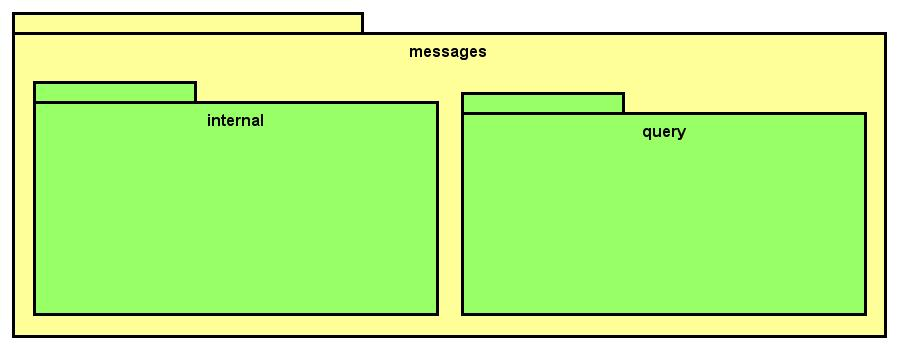
\includegraphics[scale=0.5]{Server/messagesLevel.jpg}
			\caption{Componente Actorbase.server.messages}
		\end{figure}
		La componente messages di \emph{Actorbase} è la raccolta di tutti i messaggi che vengono scambiati tra attori. Comprende sia i messaggi interni al sistema che i messaggi che rappresentano le richieste di un utente.
		
	\subsection{Actorbase.server.messages.internal}
		\begin{figure}[H]
			\centering
			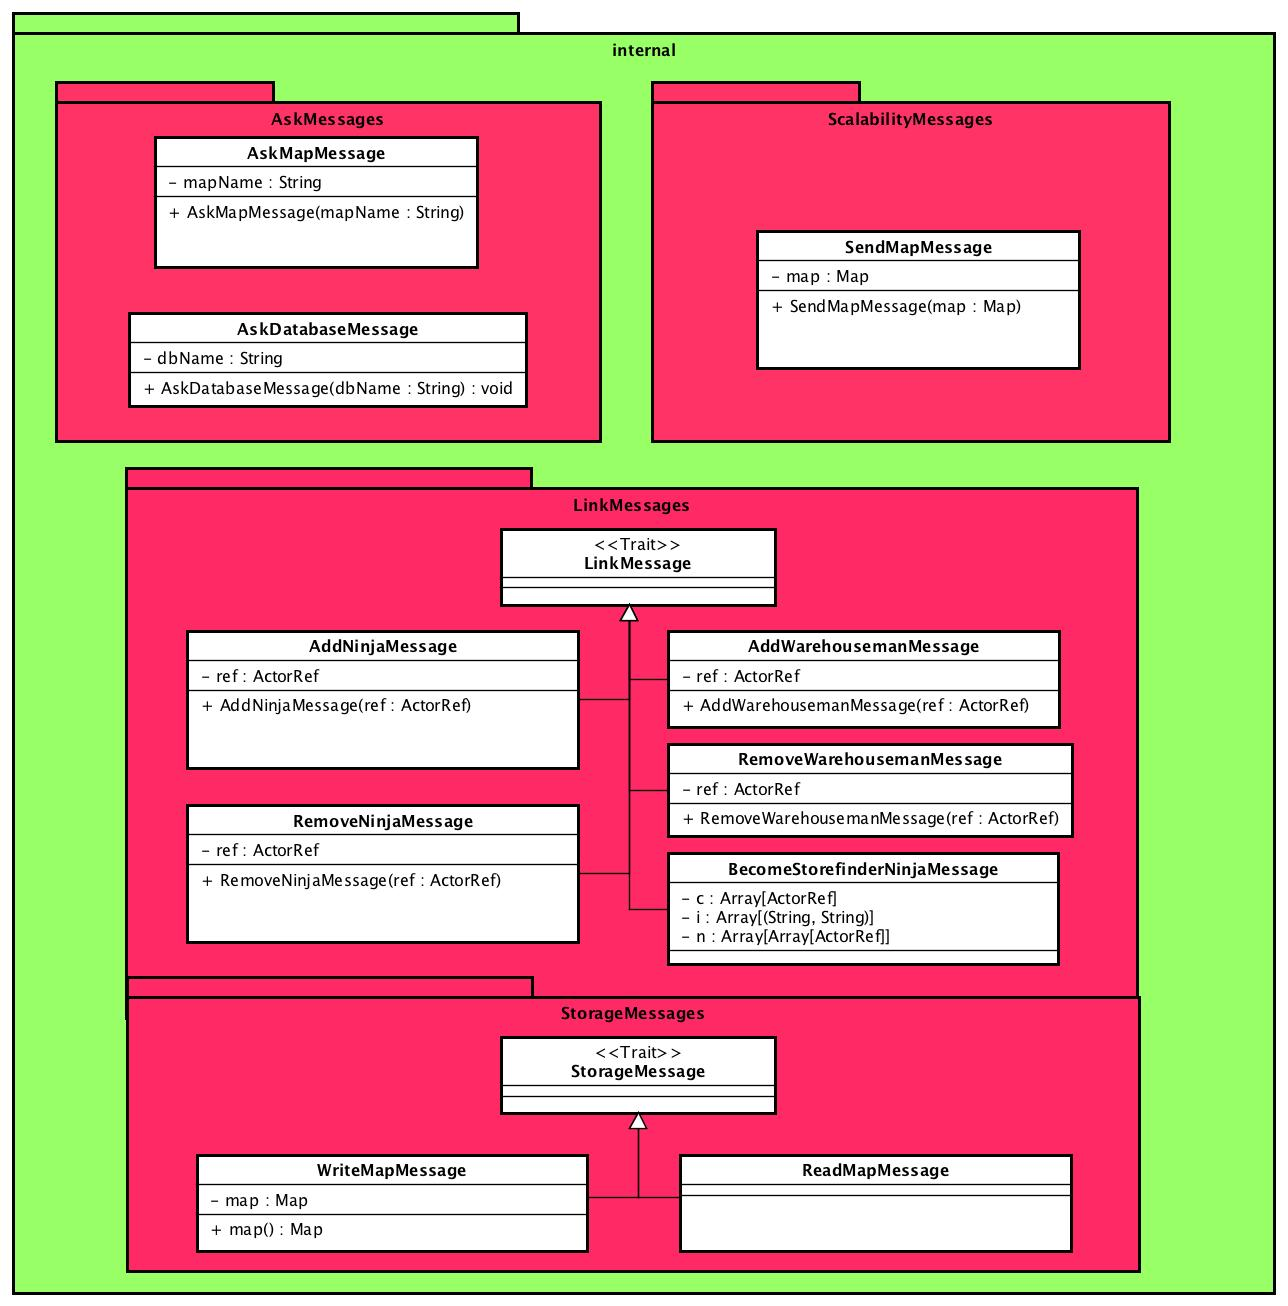
\includegraphics[scale=0.5]{Server/internalLevel.jpg}
			\caption{Componente Actorbase.server.messages.internal}
		\end{figure}
		La componente internal di \emph{Actorbase} è la raccolta dei messaggi che vengono scambiati tra attori internamente al sistema, ovvero non sono collegati direttamente ad azione dell'utente. Svolgono attività di configurazione e influenzano il comportamento degli attori.
		
	\subsection{Actorbase.server.messages.internal.AskMessages (object)}
		\textbf{Descrizione}
			\\ \\
			Un \texttt{AskMessage} definisce una richiesta di controllo dell'esistenza di un elemento.
			\\ \\
		\textbf{Utilizzo}
			\\ \\
			Messaggi di questo tipo sono utilizzati per controllare se un elemento (un database, una mappa, ...) è presente.
			\\ \\
		\textbf{Classi ereditate}
			\\ \\
			Nessuna.
			\\ \\
		\textbf{Ereditata da}
			\\ \\
			Nessuno.
			\\ \\
		\textbf{Attributi}
			\\ \\
			Nessuno.
			\\ \\
		\textbf{Metodi}
			\\ \\
			Nessuno.		
		
	\subsection{Actorbase.server.messages.internal.AskMapMessage}
		\textbf{Descrizione}
			\\ \\
			Un \texttt{AskMapMessage} definisce una richiesta di controllo dell'esistenza di una mappa.
			\\ \\
		\textbf{Utilizzo}
			\\ \\
			Messaggi di questo tipo sono utilizzati per controllare se una mappa è presente.
			\\ \\
		\textbf{Classi ereditate}
			\\ \\
			Nessuna.
			\\ \\
		\textbf{Ereditata da}
			\\ \\
			Nessuno.
			\\ \\
		\textbf{Attributi}
			\begin{itemize}
				\item \texttt{val mapName: String} - Il nome della mappa di cui si vuole controllare l'esistenza.
			\end{itemize}
		\textbf{Costruttore:} \texttt{AskMapMessage(mapName:String)}
		\\ \\
		Costruisce un \texttt{AskMapMessage} a partire dalla stringa contenente il nome della mappa.
		\\ \\
		Lista parametri del metodo:
		\begin{itemize}
			\item \texttt{mapName: String} - Il nome della mappa.
		\end{itemize}
		
	\subsection{Actorbase.server.messages.internal.AskDatabaseMessage}
		\textbf{Descrizione}
			\\ \\
			Un \texttt{AskDatabaseMessage} definisce una richiesta di controllo dell'esistenza di un database.
			\\ \\
		\textbf{Utilizzo}
			\\ \\
			Messaggi di questo tipo sono utilizzati per controllare se un database è presente.
			\\ \\
		\textbf{Classi ereditate}
			\\ \\
			Nessuna.
			\\ \\
		\textbf{Ereditata da}
			\\ \\
			Nessuno.
			\\ \\
		\textbf{Attributi}
			\begin{itemize}
				\item \texttt{val dbName: String} - Il nome del database di cui si vuole controllare l'esistenza.
			\end{itemize}
		\textbf{Costruttore:} \texttt{AskDatabaseMessage(dbName: String)}
		\\ \\
		Costruisce un \texttt{AskDatabaseMessage} a partire dalla stringa contenente il nome del database.
		\\ \\
		Lista parametri del metodo:
		\begin{itemize}
			\item \texttt{dbName: String} - Il nome del database.
		\end{itemize}
			
			
	\subsection{Actorbase.server.messages.internal.LinkMessages}
		I LinkMessages sono i messaggi usati per gestire i collegamenti tra attori. Questo tipo di messaggi deve contenere il riferimento all'attore che deve essere aggiunto o eliminato dalla mappa degli attori conosciuti. 
		
	\subsection{Actorbase.server.messages.internal.LinkMessages.LinkMessage (trait)}
		\textbf{Descrizione}
			\\ \\
			Trait che ogni messaggio che definisce operazioni di collegamento tra attori deve estendere.
			\\ \\
		\textbf{Utilizzo}
			\\ \\
			Viene utilizzato per fornire un'interfaccia comune per quanto riguarda la gestione di messaggi che riguardano il collegamento tra attori.
			\\ \\
		\textbf{Classi ereditate}
			\\ \\
			Nessuna.
			\\ \\
		\textbf{Ereditata da}
			\begin{itemize}
				\item \texttt{Actorbase.server.messages.internal.LinkMessages.AddNinjaMessage}
				\item \texttt{Actorbase.server.messages.internal.LinkMessages.AddWarehousemanMessage}
				\item \texttt{Actorbase.server.messages.internal.LinkMessages.RemoveNinjaMessage}
				\item \texttt{Actorbase.server.messages.internal.LinkMessages.RemoveWarehousemanMessage}
				\item \texttt{Actorbase.server.messages.internal.LinkMessages.BecomeStorefinderNinjaMessage}
			\end{itemize}
		\textbf{Attributi}
			\\ \\
			Nessuno.
			\\ \\
		\textbf{Metodi}
			\\ \\
			Nessuno.
			
	\subsection{Actorbase.server.messages.internal.LinkMessages.AddNinjaMessage}
		\textbf{Descrizione}
			\\ \\
			Un \texttt{AddNinjaMessage} definisce una richiesta di aggiunta di un attore di tipo \texttt{Ninja}.
			\\ \\
		\textbf{Utilizzo}
			\\ \\
			Viene utilizzato per richiedere l'aggiunta di un attore di tipo \texttt{Ninja}.
			\\ \\
		\textbf{Classi ereditate}
			\begin{itemize}
				\item \texttt{Actorbase.server.messages.internal.LinkMessages.LinkMessage}
			\end{itemize}
		\textbf{Ereditata da}
			\\ \\
			Nessuno.
			\\ \\
		\textbf{Attributi}
			\begin{itemize}
				\item \texttt{val ref : ActorRef} - Il riferimento all'attore.
			\end{itemize}
		\textbf{Costruttore:} \texttt{AddNinjaMessage(ref : ActorRef)}
		\\ \\
		Costruisce un \texttt{AddNinjaMessage} a partire dal riferimento all'attore.
		\\ \\
		Lista parametri del metodo:
			\begin{itemize}
				\item \texttt{ref : ActorRef} - Il riferimento all'attore.
			\end{itemize}
			
	\subsection{Actorbase.server.messages.internal.LinkMessages.AddWarehousemanMessage}
		\textbf{Descrizione}
			\\ \\
			Un \texttt{AddWarehousemanMessage} definisce una richiesta di aggiunta di un attore di tipo \texttt{Warehouseman}.
			\\ \\
		\textbf{Utilizzo}
			\\ \\
			Viene utilizzato per richiedere l'aggiunta di un attore di tipo \texttt{Warehouseman}.
			\\ \\
		\textbf{Classi ereditate}
			\begin{itemize}
				\item \texttt{Actorbase.server.messages.internal.LinkMessages.LinkMessage}
			\end{itemize}
		\textbf{Ereditata da}
			\\ \\
			Nessuno.
			\\ \\
		\textbf{Attributi}
			\begin{itemize}
				\item \texttt{val ref : ActorRef} - Il riferimento all'attore.
			\end{itemize}
		\textbf{Costruttore:} \texttt{AddWarehousemanMessage(ref : ActorRef)}
		\\ \\
		Costruisce un \texttt{AddWarehousemanMessage} a partire dal riferimento all'attore.
		\\ \\
		Lista parametri del metodo:
			\begin{itemize}
				\item \texttt{ref : ActorRef} - Il riferimento all'attore.
			\end{itemize}
			
	\subsection{Actorbase.server.messages.internal.LinkMessages.RemoveNinjaMessage}
		\textbf{Descrizione}
			\\ \\
			Un \texttt{RemoveNinjaMessage} definisce una richiesta di rimozione di un attore di tipo \texttt{Ninja}.
			\\ \\
		\textbf{Utilizzo}
			\\ \\
			Viene utilizzato per richiedere la rimozione di un attore di tipo \texttt{Ninja}.
			\\ \\
		\textbf{Classi ereditate}
			\begin{itemize}
				\item \texttt{Actorbase.server.messages.internal.LinkMessages.LinkMessage}
			\end{itemize}
		\textbf{Ereditata da}
			\\ \\
			Nessuno.
			\\ \\
		\textbf{Attributi}
			\begin{itemize}
				\item \texttt{val ref : ActorRef} - Il riferimento all'attore.
			\end{itemize}
		\textbf{Costruttore:} \texttt{RemoveNinjaMessage(ref : ActorRef)}
		\\ \\
		Costruisce un \texttt{RemoveNinjaMessage} a partire dal riferimento all'attore.
		\\ \\
		Lista parametri del metodo:
			\begin{itemize}
				\item \texttt{ref : ActorRef} - Il riferimento all'attore.
			\end{itemize}
			
	\subsection{Actorbase.server.messages.internal.LinkMessages.RemoveWarehousemanMessage}
		\textbf{Descrizione}
			\\ \\
			Un \texttt{RemoveWarehousemanMessage} definisce una richiesta di rimozione di un attore di tipo \texttt{Warehouseman}.
			\\ \\
		\textbf{Utilizzo}
			\\ \\
			Viene utilizzato per richiedere la rimozione di un attore di tipo \texttt{Warehouseman}.
			\\ \\
		\textbf{Classi ereditate}
			\begin{itemize}
				\item \texttt{Actorbase.server.messages.internal.LinkMessages.LinkMessage}
			\end{itemize}
		\textbf{Ereditata da}
			\\ \\
			Nessuno.
			\\ \\
		\textbf{Attributi}
			\begin{itemize}
				\item \texttt{val ref : ActorRef} - Il riferimento all'attore.
			\end{itemize}
		\textbf{Costruttore:} \texttt{RemoveWarehousemanMessage(ref : ActorRef)}
		\\ \\
		Costruisce un \texttt{RemoveWarehousemanMessage} a partire dal riferimento all'attore.
		\\ \\
		Lista parametri del metodo:
			\begin{itemize}
				\item \texttt{ref : ActorRef} - Il riferimento all'attore.
			\end{itemize}
			
	\subsection{Actorbase.server.messages.internal.LinkMessages.BecomeStorefinderNinjaMessage}
		\textbf{Descrizione}
			\\ \\
			Un \texttt{BecomeStorefinderNinjaMessage} definisce una richiesta di cambiamento del comportamento di uno \texttt{Storemanager} in \texttt{StorefinderNinja}.
			\\ \\
		\textbf{Utilizzo}
			\\ \\
			Viene utilizzato da un attore \texttt{Storemanager} quando cambia comportamento e passa da \texttt{Storekeeper} a \texttt{Storefinder}, serve ad informare i suoi ninja del cambio.
			\\ \\
		\textbf{Classi ereditate}
			\begin{itemize}
				\item \texttt{Actorbase.server.messages.internal.LinkMessages.LinkMessage}
			\end{itemize}
		\textbf{Ereditata da}
			\\ \\
			Nessuno.
			\\ \\
		\textbf{Attributi}
			\begin{itemize}
				\item \texttt{val c : Array[ActorRef]} - I riferimenti agli attori figli dello \texttt{Storefinder} originale.
				\item \texttt{val i : Array[(String, String)]} - I riferimenti agli indici degli attori figli dello \texttt{Storefinder} originale.
				\item \texttt{val n : Array[Array[ActorRef]]} - I riferimenti ai ninja degli attori figli dello \texttt{Storefinder} originale.
			\end{itemize}
		\textbf{Costruttore:} \texttt{BecomeStorefinderNinjaMessage(c : Array[ActorRef], i : Array[(String, String)], n : Array[Array[ActorRef]])}
		\\ \\
		Costruisce un \texttt{BecomeStorefinderNinjaMessage} a partire dai dati rappresentanti i figli dello \texttt{Storefinder} originale.
		\\ \\
		Lista parametri del metodo:
			\begin{itemize}
				\item \texttt{c : Array[ActorRef]} - I riferimenti agli attori figli dello \texttt{Storefinder} originale.
				\item \texttt{i : Array[(String, String)]} - I riferimenti agli indici degli attori figli dello \texttt{Storefinder} originale.
				\item \texttt{n : Array[Array[ActorRef]]} - I riferimenti ai ninja degli attori figli dello \texttt{Storefinder} originale.
			\end{itemize}
			
	\subsection{Actorbase.server.messages.internal.ScalabilityMessages}
		Gli ScalabilityMessages sono messaggi usati per gestire le proprietà di scalabilità del sistema.
		
	\subsection{Actorbase.server.messages.internal.ScalabilityMessages.ScalabilityMessage (trait)}
		\textbf{Descrizione}
			\\ \\
			Trait che ogni messaggio che definisce operazioni relative alla scalabilità del sistema deve estendere.
			\\ \\
		\textbf{Utilizzo}
			\\ \\
			Viene utilizzato per fornire un'interfaccia comune per quanto riguarda la gestione di messaggi che riguardano la scalabilità del sistema.
			\\ \\
		\textbf{Classi ereditate}
			\\ \\
			Nessuna.
			\\ \\
		\textbf{Ereditata da}
			\begin{itemize}
				\item \texttt{Actorbase.server.messages.internal.ScalabilityMessages.SendMapMessage}
			\end{itemize}
		\textbf{Attributi}
			\\ \\
			Nessuno.
			\\ \\
		\textbf{Metodi}
			\\ \\
			Nessuno.
			
	\subsection{Actorbase.server.messages.internal.ScalabilityMessages.SendMapMessage}
		\textbf{Descrizione}
			\\ \\
			Messaggio che definisce una richiesta di aggiunta di una mappa ad un attore preesistente.
			\\ \\
		\textbf{Utilizzo}
			\\ \\
			Viene utilizzato per passare mappe tra attori.
			\\ \\
		\textbf{Classi ereditate}
			\begin{itemize}
				\item \texttt{Actorbase.server.messages.internal.ScalabilityMessages.ScalabilityMessage}
			\end{itemize}
		\textbf{Ereditata da}
			\\ \\
			Nessuno.
			\\ \\
		\textbf{Attributi}
			\begin{itemize}
				\item \texttt{val map: mutable.HashMap[String, Array[Byte]]} -La mappa che deve essere inviata.
			\end{itemize}
		\textbf{Costruttore:} \texttt{SendMapMessage (map: mutable.HashMap[String, Array[Byte]])}
		\\ \\
		Costruisce un \texttt{SendMapMessage} a partire dalla mappa che deve essere inviata.
		\\ \\
		Lista parametri del metodo:
			\begin{itemize}
				\item \texttt{map: mutable.HashMap[String, Array[Byte]]} -La mappa che deve essere inviata.
			\end{itemize}
			
	\subsection{Actorbase.server.messages.internal.StorageMessages}
		Gli StorageMessages sono messaggi usati per effettuare operazioni relative alla gestione dei dati su file.
		
	\subsection{Actorbase.server.messages.internal.StorageMessages.StorageMessages (trait)}
		\textbf{Descrizione}
			\\ \\
			Trait che ogni messaggio che definisce operazioni relative alla gestione dei dati su disco deve estendere.
			\\ \\
		\textbf{Utilizzo}
			\\ \\
			Viene utilizzato per fornire un'interfaccia comune per quanto riguarda la gestione di messaggi che riguardano la gestione dei dati su disco
			\\ \\
		\textbf{Classi ereditate}
			\\ \\
			Nessuna.
			\\ \\
		\textbf{Ereditata da}
			\begin{itemize}
				\item \texttt{Actorbase.server.messages.internal.StorageMessages.WriteMapMessage}
				\item \texttt{Actorbase.server.messages.internal.StorageMessages.ReadMapMessage}
			\end{itemize}
		\textbf{Attributi}
			\\ \\
			Nessuno.
			\\ \\
		\textbf{Metodi}
			\\ \\
			Nessuno.
			
	\subsection{Actorbase.server.messages.internal.StorageMessages.WriteMapMessage}
		\textbf{Descrizione}
			\\ \\
			Messaggio che definisce una richiesta di scrittura di una mappa su disco.
			\\ \\
		\textbf{Utilizzo}
			\\ \\
			Viene utilizzato per scrivere una mappa su disco.
			\\ \\
		\textbf{Classi ereditate}
			\begin{itemize}
				\item \texttt{Actorbase.server.messages.internal.StorageMessages.StorageMessages}
			\end{itemize}
		\textbf{Ereditata da}
			\\ \\
			Nessuno.
			\\ \\
		\textbf{Attributi}
			\begin{itemize}
				\item \texttt{val map: mutable.HashMap[String, Array[Byte]]} -La mappa che deve essere scritta su disco.
			\end{itemize}
		\textbf{Costruttore:} \texttt{WriteMapMessage (map: HashMap[String, Array[Byte]])}
		\\ \\
		Costruisce un \texttt{WriteMapMessage} a partire dalla mappa che deve essere scritta.
		\\ \\
		Lista parametri del metodo:
			\begin{itemize}
				\item \texttt{map: mutable.HashMap[String, Array[Byte]]} -La mappa che deve essere scritta.
			\end{itemize}
			
	\subsection{Actorbase.server.messages.internal.StorageMessages.ReadMapMessage}
		\textbf{Descrizione}
			\\ \\
			Messaggio che definisce una richiesta di lettura di una mappa da disco.
			\\ \\
		\textbf{Utilizzo}
			\\ \\
			Viene utilizzato per leggere una mappa da disco.
			\\ \\
		\textbf{Classi ereditate}
			\begin{itemize}
				\item \texttt{Actorbase.server.messages.internal.StorageMessages.StorageMessages}
			\end{itemize}
		\textbf{Ereditata da}
			\\ \\
			Nessuno.
			\\ \\
		\textbf{Attributi}
			\\ \\
			Nessuno.
			\\ \\
		\textbf{Costruttore:} \texttt{ReadMapMessage()}
		\\ \\
		Costruisce un \texttt{ReadMapMessage} senza parametri.
		\\ \\
		Nessuno.
			
	\subsection{Actorbase.server.messages.query}
		\begin{figure}[H]
			\centering
			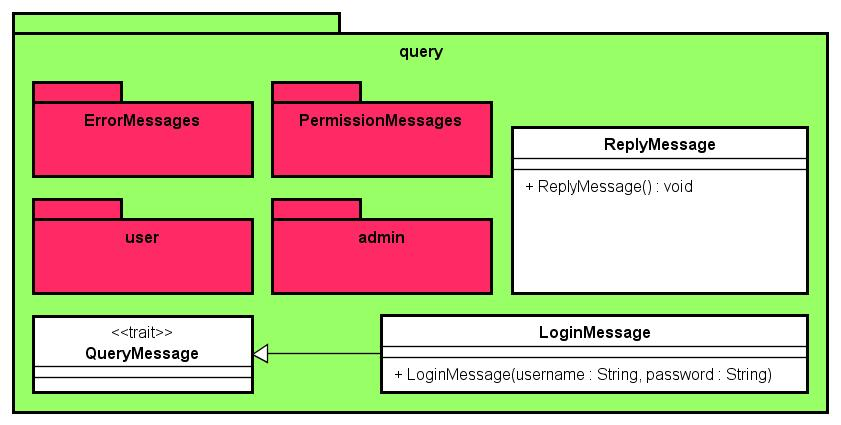
\includegraphics[scale=0.5]{Server/queryLevel.jpg}
			\caption{Componente Actorbase.server.messages.query}
		\end{figure}
		La componente query di \emph{Actorbase} raccoglie tutti i messaggi che rappresentano richieste dirette di un utente e i messaggi di risposta a tali richieste. Comprende inoltre le richieste degli amministratori.
		
	\subsection{Actorbase.server.messages.query.QueryMessage (trait)}
		\textbf{Descrizione}
			\\ \\
			Interfaccia di base dei messaggi di tipo query.
			\\ \\
		\textbf{Utilizzo}
			\\ \\
			Questa interfaccia fornisce un tipo comune per tutti i messaggi che rappresentano una query ed è estesa dai messaggi concreti.
			\\ \\
		\textbf{Classi ereditate}
			\\ \\
			Nessuna.
			\\ \\
		\textbf{Ereditata da}
			\begin{itemize}
				\item \texttt{Actorbase.server.messages.query.LoginMessage }
				\item \texttt{Actorbase.server.messages.query.user.UserMessage }
			\end{itemize}
		\textbf{Attributi}
			\\ \\
			Nessuno.
			\\ \\
		\textbf{Metodi}
			\\ \\
			Nessuno.
			
	\subsection{Actorbase.server.messages.query.ServiceErrorInfo}
		\textbf{Descrizione}
			\\ \\
			Classe che rappresenta una risposta di errore nel servizio.
			\\ \\
		\textbf{Utilizzo}
			\\ \\
			Questa classe viene utilizzata per comunicare un errore generale di servizio all'utente.
			\\ \\
		\textbf{Classi ereditate}
			\begin{itemize}
				\item \texttt{Actorbase.server.messages.ReplyErrorInfo }
			\end{itemize}
		\textbf{Ereditata da}
			\\ \\
			Nessuna.
			\\ \\
		\textbf{Attributi}
			\begin{itemize}
				\item \texttt{error: String } - Stringa che descrive l'errore da comunicare all'utente.
			\end{itemize}
		\textbf{Costruttore: } \texttt{ServiceErrorInfo(error : String)}
			\\ \\
		Metodo che costruisce un oggetto di tipo ServiceErrorInfo.
			\\ \\
		Lista parametri del metodo:
			\begin{itemize}
				\item \texttt{error: String } - Stringa che descrive l'errore da comunicare all'utente.
			\end{itemize}
		\textbf{Metodo: } \texttt{error(): String}
			\\ \\
		Metodo che ritorna l'attributo error della classe.
			\\ \\
		Lista parametri del metodo:
			\\ \\
			Nessuno.
			
	\subsection{Actorbase.server.messages.query.LoginMessage}
		\textbf{Descrizione}
			\\ \\
			Classe che rappresenta una richiesta di login da parte di un utente.
			\\ \\
		\textbf{Utilizzo}
			\\ \\
			Questa classe è un messaggio che viene creato quando viene riconosciuta una richiesta di login dal parser e serve a controllare le credenziali dell'utente che vuole accedere al sistema.
			\\ \\
		\textbf{Classi ereditate}
			\begin{itemize}
				\item \texttt{Actorbase.server.messages.query.QueryMessage }
			\end{itemize}
		\textbf{Ereditata da}
			\\ \\
			Nessuna.
			\\ \\
		\textbf{Attributi}
			\begin{itemize}
				\item \texttt{username: String } - Username dell'utente che richiede di accedere al sistema.
				\item \texttt{password: String } - Password dell'utente che richiede di accedere al sistema.
			\end{itemize}
		\textbf{Costruttore: } \texttt{LoginMessage(username: String, password: String)}
			\\ \\
		Metodo che costruisce un oggetto di tipo LoginMessage.
			\\ \\
		Lista parametri del metodo:
			\begin{itemize}
				\item \texttt{username: String } - Username dell'utente che richiede di accedere al sistema.
				\item \texttt{password: String } - Password dell'utente che richiede di accedere al sistema.
			\end{itemize}
		\textbf{Metodo: } \texttt{username(): String}
			\\ \\
		Metodo che ritorna l'attributo username della classe.
			\\ \\
		Lista parametri del metodo:
			\\ \\
			Nessuno.
			\\ \\		
		\textbf{Metodo: } \texttt{password(): String}
			\\ \\
		Metodo che ritorna l'attributo password della classe.
			\\ \\
		Lista parametri del metodo:
			\\ \\
			Nessuno.
	
	\subsection{Actorbase.server.messages.query.ReplyInfo (trait)}
			\textbf{Descrizione}
			\\ \\
			Interfaccia di base dei messaggi di tipo ReplyInfo.
			\\ \\
		\textbf{Utilizzo}
			\\ \\
			Questa interfaccia fornisce un tipo comune per tutti i messaggi che rappresentano informazioni aggiuntive sul risultato di una query dell'utente.
			\\ \\
		\textbf{Classi ereditate}
			\\ \\
			Nessuna.
			\\ \\
		\textbf{Ereditata da}
			\begin{itemize}
				\item \texttt{Actorbase.server.messages.query.ReplyErrorInfo }
				\item \texttt{Actorbase.server.messages.query.ServiceErrorInfo }
				\item \texttt{Actorbase.server.messages.query.ErrorMessages.QueryErrorInfo }
				\item \texttt{Actorbase.server.messages.query.PermissionMessages.NoReadPermissionInfo }
  				\item \texttt{Actorbase.server.messages.query.PermissionMessages.NoWritePermissionInfo }
  				\item \texttt{Actorbase.server.messages.query.PermissionMessages.NoAdminPermissionInfo }
  				\item \texttt{Actorbase.server.messages.query.admin.PermissionManagementMessages.ListPermissionsInfo }
  				\item \texttt{Actorbase.server.messages.query.admin.UsersManagementMessages.ListUserInfo }
  				\item \texttt{Actorbase.server.messages.query.admin.UsersManagementMessages.NoUserInfo }
  				\item \texttt{Actorbase.server.messages.query.admin.UsersManagementMessages.AddUserInfo }
  				\item \texttt{Actorbase.server.messages.query.admin.UsersManagementMessages.RemoveUserInfo }
  				\item \texttt{Actorbase.server.messages.query.user.RowMessages.KeyAlreadyExistInfo }
  				\item \texttt{Actorbase.server.messages.query.user.RowMessages.KeyDoesNotExistInfo }
  				\item \texttt{Actorbase.server.messages.query.user.RowMessages.ListKeyInfo }
  				\item \texttt{Actorbase.server.messages.query.user.RowMessages.NoKeyInfo }
  				\item \texttt{Actorbase.server.messages.query.user.RowMessages.FindInfo }
  				\item \texttt{Actorbase.server.messages.query.user.DatabaseMessages.DBAlreadyExistInfo }
  				\item \texttt{Actorbase.server.messages.query.user.DatabaseMessages.DBDoesNotExistInfo }
  				\item \texttt{Actorbase.server.messages.query.user.DatabaseMessages.ListDBInfo }
  				\item \texttt{Actorbase.server.messages.query.user.DatabaseMessages.NoDBInfo }
  				\item \texttt{Actorbase.server.messages.query.user.DatabaseMessages.NoDBSelectedInfo }
  				\item \texttt{Actorbase.server.messages.query.user.HelpMessages.CompleteHelpReplyInfo }
  				\item \texttt{Actorbase.server.messages.query.user.HelpMessages.SpecificHelpReplyInfo }
  				\item \texttt{Actorbase.server.messages.query.user.MapMessages.MapAlreadyExistInfo }
  				\item \texttt{Actorbase.server.messages.query.user.MapMessages.MapDoesNotExistInfo }
  				\item \texttt{Actorbase.server.messages.query.user.MapMessages.ListMapInfo }
  				\item \texttt{Actorbase.server.messages.query.user.MapMessages.NoMapInfo }
  				\item \texttt{Actorbase.server.messages.query.user.MapMessages.NoMapSelectedInfo }
			\end{itemize}
		\textbf{Attributi}
			\\ \\
			Nessuno.
			\\ \\
		\textbf{Metodi}
			\\ \\
			Nessuno.
		
	\subsection{Actorbase.server.messages.query.ReplyErrorInfo}
		\textbf{Descrizione}
			\\ \\
			Classe che rappresenta una risposta di errore generale.
			\\ \\
		\textbf{Utilizzo}
			\\ \\
			Questa classe viene utilizzata per rappresentare un errore generale e comunicarlo all'utente.
			\\ \\
		\textbf{Classi ereditate}
			\\ \\
			Nessuna.
			\\ \\
		\textbf{Ereditata da}
			\begin{itemize}
				\item \texttt{Actorbase.server.messages.ServiceErrorInfo }
			\end{itemize}
		\textbf{Attributi}
			\\ \\
			Nessuno.
			\\ \\
		\textbf{Metodi}
			\\ \\
			Nessuno.
					
	\subsection{Actorbase.server.messages.query.ReplyMessage}
		\textbf{Descrizione}
			\\ \\
			Classe che rappresenta la risposta ad una richiesta dell'utente.
			\\ \\
		\textbf{Utilizzo}
			\\ \\
			Questa classe viene creata con le informazioni necessarie per rispondere all'utente in merito ad una richiesta.
			\\ \\
		\textbf{Classi ereditate}
			\\ \\
			Nessuna.
			\\ \\
		\textbf{Ereditata da}
			\\ \\
			Nessuna.
			\\ \\
		\textbf{Attributi}
			\begin{itemize}
				\item \texttt{result: ReplyResult } - Esito della query.
				\item \texttt{question: QueryMessage } - La query a cui rispondere.
				\item \texttt{info: ReplyInfo = null } - Risultato della query, contenente i dati richiesti.
			\end{itemize}
			\textbf{Costruttore: } \texttt{ReplyMessage(result: ReplyResult, question: QueryMessage, info: ReplyInfo = null)}
			\\ \\
			Metodo che costruisce un oggetto di tipo ReplyResult.
			\\ \\
			Lista parametri del metodo:
			\begin{itemize}
				\item \texttt{result: ReplyResult } - Esito della query.
				\item \texttt{question: QueryMessage } - La query a cui rispondere.
				\item \texttt{info: ReplyInfo = null } - Risultato della query, contenente i dati richiesti.
			\end{itemize}
			\textbf{Metodo: } \texttt{result(): ReplyResult }
			\\ \\
			Metodo che ritorna l'attributo result della classe.
			\\ \\
			Lista parametri del metodo:
			\\ \\
			Nessuno.
			\\ \\		
			\textbf{Metodo: } \texttt{question(): QueryMessage}
			\\ \\
			Metodo che ritorna l'attributo question della classe.
			\\ \\
			Lista parametri del metodo:
			\\ \\
			Nessuno.
			\\ \\
			\textbf{Metodo: } \texttt{info(): ReplyInfo}
			\\ \\	
			Metodo che ritorna l'attributo info della classe.
			\\ \\
			Lista parametri del metodo:
			\\ \\
			Nessuno.
			\\ \\
			
	\subsection{Actorbase.server.messages.query.ErrorMessages}
		Immagine UML del package e breve descrizione.
		
	\subsection{Actorbase.server.messages.query.ErrorMessages.ErrorMessage (trait)}
		Immagine UML.
		\\ \\
		\textbf{Descrizione}
			\\ \\
			Descrizione testuale.
			\\ \\
		\textbf{Utilizzo}
			\\ \\
			Descrizione testuale.
			\\ \\
		\textbf{Classi ereditate}
			\begin{itemize}
				\item Classe
				\item \dots
			\end{itemize}
		\textbf{Ereditata da}
			\begin{itemize}
				\item Classe
				\item \dots
			\end{itemize}
		\textbf{Attributi}
			\begin{itemize}
				\item \texttt{Nome attributo: tipo attributo } - Descrizione attributo
				\item \dots
			\end{itemize}
		\textbf{Metodi}
			\\ \\
			Nessuno.
			
	\subsection{Actorbase.server.messages.query.ErrorMessages.InvalidQueryMessage}
		Immagine UML.
		\\ \\
		\textbf{Descrizione}
			\\ \\
			Descrizione testuale.
			\\ \\
		\textbf{Utilizzo}
			\\ \\
			Descrizione testuale.
			\\ \\
		\textbf{Classi ereditate}
			\begin{itemize}
				\item Classe
				\item \dots
			\end{itemize}
		\textbf{Ereditata da}
			\begin{itemize}
				\item Classe
				\item \dots
			\end{itemize}
		\textbf{Attributi}
			\begin{itemize}
				\item \texttt{Nome attributo: tipo attributo } - Descrizione attributo
				\item \dots
			\end{itemize}
		\textbf{Metodi}
			\\ \\
			Nessuno.
			
	\subsection{Actorbase.server.messages.query.PermissionMessages}
		Immagine UML del package e breve descrizione.
		
	\subsection{Actorbase.server.messages.query.PermissionMessages.AdminPermissionMessage (trait)}
		Immagine UML.
		\\ \\
		\textbf{Descrizione}
			\\ \\
			Descrizione testuale.
			\\ \\
		\textbf{Utilizzo}
			\\ \\
			Descrizione testuale.
			\\ \\
		\textbf{Classi ereditate}
			\begin{itemize}
				\item Classe
				\item \dots
			\end{itemize}
		\textbf{Ereditata da}
			\begin{itemize}
				\item Classe
				\item \dots
			\end{itemize}
		\textbf{Attributi}
			\begin{itemize}
				\item \texttt{Nome attributo: tipo attributo } - Descrizione attributo
				\item \dots
			\end{itemize}
		\textbf{Metodi}
			\\ \\
			Nessuno.
			
\subsection{Actorbase.server.messages.query.PermissionMessages.NoPermissionMessage (trait)}
		Immagine UML.
		\\ \\
		\textbf{Descrizione}
			\\ \\
			Descrizione testuale.
			\\ \\
		\textbf{Utilizzo}
			\\ \\
			Descrizione testuale.
			\\ \\
		\textbf{Classi ereditate}
			\begin{itemize}
				\item Classe
				\item \dots
			\end{itemize}
		\textbf{Ereditata da}
			\begin{itemize}
				\item Classe
				\item \dots
			\end{itemize}
		\textbf{Attributi}
			\begin{itemize}
				\item \texttt{Nome attributo: tipo attributo } - Descrizione attributo
				\item \dots
			\end{itemize}
		\textbf{Metodi}
			\\ \\
			Nessuno.
			
\subsection{Actorbase.server.messages.query.PermissionMessages.ReadMessage (trait)}
		Immagine UML.
		\\ \\
		\textbf{Descrizione}
			\\ \\
			Descrizione testuale.
			\\ \\
		\textbf{Utilizzo}
			\\ \\
			Descrizione testuale.
			\\ \\
		\textbf{Classi ereditate}
			\begin{itemize}
				\item Classe
				\item \dots
			\end{itemize}
		\textbf{Ereditata da}
			\begin{itemize}
				\item Classe
				\item \dots
			\end{itemize}
		\textbf{Attributi}
			\begin{itemize}
				\item \texttt{Nome attributo: tipo attributo } - Descrizione attributo
				\item \dots
			\end{itemize}
		\textbf{Metodi}
			\\ \\
			Nessuno.
			
\subsection{Actorbase.server.messages.query.PermissionMessages.ReadWriteMessage (trait)}
		Immagine UML.
		\\ \\
		\textbf{Descrizione}
			\\ \\
			Descrizione testuale.
			\\ \\
		\textbf{Utilizzo}
			\\ \\
			Descrizione testuale.
			\\ \\
		\textbf{Classi ereditate}
			\begin{itemize}
				\item Classe
				\item \dots
			\end{itemize}
		\textbf{Ereditata da}
			\begin{itemize}
				\item Classe
				\item \dots
			\end{itemize}
		\textbf{Attributi}
			\begin{itemize}
				\item \texttt{Nome attributo: tipo attributo } - Descrizione attributo
				\item \dots
			\end{itemize}
		\textbf{Metodi}
			\\ \\
			Nessuno.
			
	\subsection{Actorbase.server.messages.query.admin}
		Immagine UML del package e breve descrizione.
		
\subsection{Actorbase.server.messages.query.admin.AdminMessage (trait)}
		Immagine UML.
		\\ \\
		\textbf{Descrizione}
			\\ \\
			Descrizione testuale.
			\\ \\
		\textbf{Utilizzo}
			\\ \\
			Descrizione testuale.
			\\ \\
		\textbf{Classi ereditate}
			\begin{itemize}
				\item Classe
				\item \dots
			\end{itemize}
		\textbf{Ereditata da}
			\begin{itemize}
				\item Classe
				\item \dots
			\end{itemize}
		\textbf{Attributi}
			\begin{itemize}
				\item \texttt{Nome attributo: tipo attributo } - Descrizione attributo
				\item \dots
			\end{itemize}
		\textbf{Metodi}
			\\ \\
			Nessuno.
		
	\subsection{Actorbase.server.messages.query.admin.ActorPropertiesMessages}
		Immagine UML del package e breve descrizione.
		
\subsection{Actorbase.server.messages.query.admin.ActorPropertiesMessages.ActorPropertiesMessage (trait)}
		Immagine UML.
		\\ \\
		\textbf{Descrizione}
			\\ \\
			Descrizione testuale.
			\\ \\
		\textbf{Utilizzo}
			\\ \\
			Descrizione testuale.
			\\ \\
		\textbf{Classi ereditate}
			\begin{itemize}
				\item Classe
				\item \dots
			\end{itemize}
		\textbf{Ereditata da}
			\begin{itemize}
				\item Classe
				\item \dots
			\end{itemize}
		\textbf{Attributi}
			\begin{itemize}
				\item \texttt{Nome attributo: tipo attributo } - Descrizione attributo
				\item \dots
			\end{itemize}
		\textbf{Metodi}
			\\ \\
			Nessuno.
			
\subsection{Actorbase.server.messages.query.admin.ActorPropertiesMessages.MaxRowMessage}
		Immagine UML.
		\\ \\
		\textbf{Descrizione}
			\\ \\
			Descrizione testuale.
			\\ \\
		\textbf{Utilizzo}
			\\ \\
			Descrizione testuale.
			\\ \\
		\textbf{Classi ereditate}
			\begin{itemize}
				\item Classe
				\item \dots
			\end{itemize}
		\textbf{Ereditata da}
			\begin{itemize}
				\item Classe
				\item \dots
			\end{itemize}
		\textbf{Attributi}
			\begin{itemize}
				\item \texttt{Nome attributo: tipo attributo } - Descrizione attributo
				\item \dots
			\end{itemize}
		\textbf{Metodi}
			\\ \\
			Nessuno.
			
\subsection{Actorbase.server.messages.query.admin.ActorPropertiesMessages.MaxRowMessage}
		Immagine UML.
		\\ \\
		\textbf{Descrizione}
			\\ \\
			Descrizione testuale.
			\\ \\
		\textbf{Utilizzo}
			\\ \\
			Descrizione testuale.
			\\ \\
		\textbf{Classi ereditate}
			\begin{itemize}
				\item Classe
				\item \dots
			\end{itemize}
		\textbf{Ereditata da}
			\begin{itemize}
				\item Classe
				\item \dots
			\end{itemize}
		\textbf{Attributi}
			\begin{itemize}
				\item \texttt{Nome attributo: tipo attributo } - Descrizione attributo
				\item \dots
			\end{itemize}
		\textbf{Metodi}
			\\ \\
			Nessuno.
			
\subsection{Actorbase.server.messages.query.admin.ActorPropertiesMessages.SetNinjaMessage}
		Immagine UML.
		\\ \\
		\textbf{Descrizione}
			\\ \\
			Descrizione testuale.
			\\ \\
		\textbf{Utilizzo}
			\\ \\
			Descrizione testuale.
			\\ \\
		\textbf{Classi ereditate}
			\begin{itemize}
				\item Classe
				\item \dots
			\end{itemize}
		\textbf{Ereditata da}
			\begin{itemize}
				\item Classe
				\item \dots
			\end{itemize}
		\textbf{Attributi}
			\begin{itemize}
				\item \texttt{Nome attributo: tipo attributo } - Descrizione attributo
				\item \dots
			\end{itemize}
		\textbf{Metodi}
			\\ \\
			Nessuno.			
			
\subsection{Actorbase.server.messages.query.admin.ActorPropertiesMessages.MaxNinjaMessage}
		Immagine UML.
		\\ \\
		\textbf{Descrizione}
			\\ \\
			Descrizione testuale.
			\\ \\
		\textbf{Utilizzo}
			\\ \\
			Descrizione testuale.
			\\ \\
		\textbf{Classi ereditate}
			\begin{itemize}
				\item Classe
				\item \dots
			\end{itemize}
		\textbf{Ereditata da}
			\begin{itemize}
				\item Classe
				\item \dots
			\end{itemize}
		\textbf{Attributi}
			\begin{itemize}
				\item \texttt{Nome attributo: tipo attributo } - Descrizione attributo
				\item \dots
			\end{itemize}
		\textbf{Metodi}
			\\ \\
			Nessuno.
			
\subsection{Actorbase.server.messages.query.admin.ActorPropertiesMessages.
\newline SetWarehousemanMessage}
		Immagine UML.
		\\ \\
		\textbf{Descrizione}
			\\ \\
			Descrizione testuale.
			\\ \\
		\textbf{Utilizzo}
			\\ \\
			Descrizione testuale.
			\\ \\
		\textbf{Classi ereditate}
			\begin{itemize}
				\item Classe
				\item \dots
			\end{itemize}
		\textbf{Ereditata da}
			\begin{itemize}
				\item Classe
				\item \dots
			\end{itemize}
		\textbf{Attributi}
			\begin{itemize}
				\item \texttt{Nome attributo: tipo attributo } - Descrizione attributo
				\item \dots
			\end{itemize}
		\textbf{Metodi}
			\\ \\
			Nessuno.			
			
\subsection{Actorbase.server.messages.query.admin.ActorPropertiesMessages.
\newline MaxWarehousemanMessage}
		Immagine UML.
		\\ \\
		\textbf{Descrizione}
			\\ \\
			Descrizione testuale.
			\\ \\
		\textbf{Utilizzo}
			\\ \\
			Descrizione testuale.
			\\ \\
		\textbf{Classi ereditate}
			\begin{itemize}
				\item Classe
				\item \dots
			\end{itemize}
		\textbf{Ereditata da}
			\begin{itemize}
				\item Classe
				\item \dots
			\end{itemize}
		\textbf{Attributi}
			\begin{itemize}
				\item \texttt{Nome attributo: tipo attributo } - Descrizione attributo
				\item \dots
			\end{itemize}
		\textbf{Metodi}
			\\ \\
			Nessuno.
			
\subsection{Actorbase.server.messages.query.admin.ActorPropertiesMessages.MaxStorekeeperMessage}
		Immagine UML.
		\\ \\
		\textbf{Descrizione}
			\\ \\
			Descrizione testuale.
			\\ \\
		\textbf{Utilizzo}
			\\ \\
			Descrizione testuale.
			\\ \\
		\textbf{Classi ereditate}
			\begin{itemize}
				\item Classe
				\item \dots
			\end{itemize}
		\textbf{Ereditata da}
			\begin{itemize}
				\item Classe
				\item \dots
			\end{itemize}
		\textbf{Attributi}
			\begin{itemize}
				\item \texttt{Nome attributo: tipo attributo } - Descrizione attributo
				\item \dots
			\end{itemize}
		\textbf{Metodi}
			\\ \\
			Nessuno.
			
\subsection{Actorbase.server.messages.query.admin.ActorPropertiesMessages.MaxStorefinderMessage}
		Immagine UML.
		\\ \\
		\textbf{Descrizione}
			\\ \\
			Descrizione testuale.
			\\ \\
		\textbf{Utilizzo}
			\\ \\
			Descrizione testuale.
			\\ \\
		\textbf{Classi ereditate}
			\begin{itemize}
				\item Classe
				\item \dots
			\end{itemize}
		\textbf{Ereditata da}
			\begin{itemize}
				\item Classe
				\item \dots
			\end{itemize}
		\textbf{Attributi}
			\begin{itemize}
				\item \texttt{Nome attributo: tipo attributo } - Descrizione attributo
				\item \dots
			\end{itemize}
		\textbf{Metodi}
			\\ \\
			Nessuno.
			
	\subsection{Actorbase.server.messages.query.admin.PermissionsManagementMessages}
		Immagine UML del package e breve descrizione.
		
	\subsection{Actorbase.server.messages.query.admin.PermissionsManagementMessages.
	\newline PermissionManagementMessage (trait)}
		Immagine UML.
		\\ \\
		\textbf{Descrizione}
			\\ \\
			Descrizione testuale.
			\\ \\
		\textbf{Utilizzo}
			\\ \\
			Descrizione testuale.
			\\ \\
		\textbf{Classi ereditate}
			\begin{itemize}
				\item Classe
				\item \dots
			\end{itemize}
		\textbf{Ereditata da}
			\begin{itemize}
				\item Classe
				\item \dots
			\end{itemize}
		\textbf{Attributi}
			\begin{itemize}
				\item \texttt{Nome attributo: tipo attributo } - Descrizione attributo
				\item \dots
			\end{itemize}
		\textbf{Metodi}
			\\ \\
			Nessuno.
			
\subsection{Actorbase.server.messages.query.admin.PermissionsManagementMessages.
\newline AddPermissionMessage}
		Immagine UML.
		\\ \\
		\textbf{Descrizione}
			\\ \\
			Descrizione testuale.
			\\ \\
		\textbf{Utilizzo}
			\\ \\
			Descrizione testuale.
			\\ \\
		\textbf{Classi ereditate}
			\begin{itemize}
				\item Classe
				\item \dots
			\end{itemize}
		\textbf{Ereditata da}
			\begin{itemize}
				\item Classe
				\item \dots
			\end{itemize}
		\textbf{Attributi}
			\begin{itemize}
				\item \texttt{Nome attributo: tipo attributo } - Descrizione attributo
				\item \dots
			\end{itemize}
		\textbf{Metodi}
			\\ \\
			Nessuno.
			
\subsection{Actorbase.server.messages.query.admin.PermissionsManagementMessages.
\newline RemovePermissionMessage}
		Immagine UML.
		\\ \\
		\textbf{Descrizione}
			\\ \\
			Descrizione testuale.
			\\ \\
		\textbf{Utilizzo}
			\\ \\
			Descrizione testuale.
			\\ \\
		\textbf{Classi ereditate}
			\begin{itemize}
				\item Classe
				\item \dots
			\end{itemize}
		\textbf{Ereditata da}
			\begin{itemize}
				\item Classe
				\item \dots
			\end{itemize}
		\textbf{Attributi}
			\begin{itemize}
				\item \texttt{Nome attributo: tipo attributo } - Descrizione attributo
				\item \dots
			\end{itemize}
		\textbf{Metodi}
			\\ \\
			Nessuno.
			
\subsection{Actorbase.server.messages.query.admin.PermissionsManagementMessages.
\newline ListPermissionMessage}
		Immagine UML.
		\\ \\
		\textbf{Descrizione}
			\\ \\
			Descrizione testuale.
			\\ \\
		\textbf{Utilizzo}
			\\ \\
			Descrizione testuale.
			\\ \\
		\textbf{Classi ereditate}
			\begin{itemize}
				\item Classe
				\item \dots
			\end{itemize}
		\textbf{Ereditata da}
			\begin{itemize}
				\item Classe
				\item \dots
			\end{itemize}
		\textbf{Attributi}
			\begin{itemize}
				\item \texttt{Nome attributo: tipo attributo } - Descrizione attributo
				\item \dots
			\end{itemize}
		\textbf{Metodi}
			\\ \\
			Nessuno.
			
	\subsection{Actorbase.server.messages.query.admin.UserManagementMessages}
		Immagine UML del package e breve descrizione.
		
	\subsection{Actorbase.server.messages.query.admin.UserManagementMessages.UserManagementMessage (trait)}
		Immagine UML.
		\\ \\
		\textbf{Descrizione}
			\\ \\
			Descrizione testuale.
			\\ \\
		\textbf{Utilizzo}
			\\ \\
			Descrizione testuale.
			\\ \\
		\textbf{Classi ereditate}
			\begin{itemize}
				\item Classe
				\item \dots
			\end{itemize}
		\textbf{Ereditata da}
			\begin{itemize}
				\item Classe
				\item \dots
			\end{itemize}
		\textbf{Attributi}
			\begin{itemize}
				\item \texttt{Nome attributo: tipo attributo } - Descrizione attributo
				\item \dots
			\end{itemize}
		\textbf{Metodi}
			\\ \\
			Nessuno.
		
	\subsection{Actorbase.server.messages.query.admin.UserManagementMessages.AddUserMessage}
		Immagine UML.
		\\ \\
		\textbf{Descrizione}
			\\ \\
			Descrizione testuale.
			\\ \\
		\textbf{Utilizzo}
			\\ \\
			Descrizione testuale.
			\\ \\
		\textbf{Classi ereditate}
			\begin{itemize}
				\item Classe
				\item \dots
			\end{itemize}
		\textbf{Ereditata da}
			\begin{itemize}
				\item Classe
				\item \dots
			\end{itemize}
		\textbf{Attributi}
			\begin{itemize}
				\item \texttt{Nome attributo: tipo attributo } - Descrizione attributo
				\item \dots
			\end{itemize}
		\textbf{Metodi}
			\\ \\
			Nessuno.		
			
	\subsection{Actorbase.server.messages.query.admin.UserManagementMessages.RemoveUserMessage}
		Immagine UML.
		\\ \\
		\textbf{Descrizione}
			\\ \\
			Descrizione testuale.
			\\ \\
		\textbf{Utilizzo}
			\\ \\
			Descrizione testuale.
			\\ \\
		\textbf{Classi ereditate}
			\begin{itemize}
				\item Classe
				\item \dots
			\end{itemize}
		\textbf{Ereditata da}
			\begin{itemize}
				\item Classe
				\item \dots
			\end{itemize}
		\textbf{Attributi}
			\begin{itemize}
				\item \texttt{Nome attributo: tipo attributo } - Descrizione attributo
				\item \dots
			\end{itemize}
		\textbf{Metodi}
			\\ \\
			Nessuno.	
			
	\subsection{Actorbase.server.messages.query.admin.UserManagementMessages.ListUserMessage}
		Immagine UML.
		\\ \\
		\textbf{Descrizione}
			\\ \\
			Descrizione testuale.
			\\ \\
		\textbf{Utilizzo}
			\\ \\
			Descrizione testuale.
			\\ \\
		\textbf{Classi ereditate}
			\begin{itemize}
				\item Classe
				\item \dots
			\end{itemize}
		\textbf{Ereditata da}
			\begin{itemize}
				\item Classe
				\item \dots
			\end{itemize}
		\textbf{Attributi}
			\begin{itemize}
				\item \texttt{Nome attributo: tipo attributo } - Descrizione attributo
				\item \dots
			\end{itemize}
		\textbf{Metodi}
			\\ \\
			Nessuno.	
			
	\subsection{Actorbase.server.messages.query.user}
		Immagine UML del package e breve descrizione.
		
	\subsection{Actorbase.server.messages.query.user.UserMessage (trait)}
		Immagine UML.
		\\ \\
		\textbf{Descrizione}
			\\ \\
			Descrizione testuale.
			\\ \\
		\textbf{Utilizzo}
			\\ \\
			Descrizione testuale.
			\\ \\
		\textbf{Classi ereditate}
			\begin{itemize}
				\item Classe
				\item \dots
			\end{itemize}
		\textbf{Ereditata da}
			\begin{itemize}
				\item Classe
				\item \dots
			\end{itemize}
		\textbf{Attributi}
			\begin{itemize}
				\item \texttt{Nome attributo: tipo attributo } - Descrizione attributo
				\item \dots
			\end{itemize}
		\textbf{Metodi}
			\\ \\
			Nessuno.	
			
	\subsection{Actorbase.server.messages.query.user.RowMessages}
		Immagine UML del package e breve descrizione.
		
	\subsection{Actorbase.server.messages.query.user.RowMessages.RowMessage (trait)}
		Immagine UML.
		\\ \\
		\textbf{Descrizione}
			\\ \\
			Descrizione testuale.
			\\ \\
		\textbf{Utilizzo}
			\\ \\
			Descrizione testuale.
			\\ \\
		\textbf{Classi ereditate}
			\begin{itemize}
				\item Classe
				\item \dots
			\end{itemize}
		\textbf{Ereditata da}
			\begin{itemize}
				\item Classe
				\item \dots
			\end{itemize}
		\textbf{Attributi}
			\begin{itemize}
				\item \texttt{Nome attributo: tipo attributo } - Descrizione attributo
				\item \dots
			\end{itemize}
		\textbf{Metodi}
			\\ \\
			Nessuno.	
			
	\subsection{Actorbase.server.messages.query.user.RowMessages.InsertRowMessage}
		Immagine UML.
		\\ \\
		\textbf{Descrizione}
			\\ \\
			Descrizione testuale.
			\\ \\
		\textbf{Utilizzo}
			\\ \\
			Descrizione testuale.
			\\ \\
		\textbf{Classi ereditate}
			\begin{itemize}
				\item Classe
				\item \dots
			\end{itemize}
		\textbf{Ereditata da}
			\begin{itemize}
				\item Classe
				\item \dots
			\end{itemize}
		\textbf{Attributi}
			\begin{itemize}
				\item \texttt{Nome attributo: tipo attributo } - Descrizione attributo
				\item \dots
			\end{itemize}
		\textbf{Metodi}
			\\ \\
			Nessuno.	
		
	\subsection{Actorbase.server.messages.query.user.RowMessages.UpdateRowMessage}
		Immagine UML.
		\\ \\
		\textbf{Descrizione}
			\\ \\
			Descrizione testuale.
			\\ \\
		\textbf{Utilizzo}
			\\ \\
			Descrizione testuale.
			\\ \\
		\textbf{Classi ereditate}
			\begin{itemize}
				\item Classe
				\item \dots
			\end{itemize}
		\textbf{Ereditata da}
			\begin{itemize}
				\item Classe
				\item \dots
			\end{itemize}
		\textbf{Attributi}
			\begin{itemize}
				\item \texttt{Nome attributo: tipo attributo } - Descrizione attributo
				\item \dots
			\end{itemize}
		\textbf{Metodi}
			\\ \\
			Nessuno.		
			
	\subsection{Actorbase.server.messages.query.user.RowMessages.RemoveRowMessage}
		Immagine UML.
		\\ \\
		\textbf{Descrizione}
			\\ \\
			Descrizione testuale.
			\\ \\
		\textbf{Utilizzo}
			\\ \\
			Descrizione testuale.
			\\ \\
		\textbf{Classi ereditate}
			\begin{itemize}
				\item Classe
				\item \dots
			\end{itemize}
		\textbf{Ereditata da}
			\begin{itemize}
				\item Classe
				\item \dots
			\end{itemize}
		\textbf{Attributi}
			\begin{itemize}
				\item \texttt{Nome attributo: tipo attributo } - Descrizione attributo
				\item \dots
			\end{itemize}
		\textbf{Metodi}
			\\ \\
			Nessuno.	
			
	\subsection{Actorbase.server.messages.query.user.RowMessages.FindRowMessage}
		Immagine UML.
		\\ \\
		\textbf{Descrizione}
			\\ \\
			Descrizione testuale.
			\\ \\
		\textbf{Utilizzo}
			\\ \\
			Descrizione testuale.
			\\ \\
		\textbf{Classi ereditate}
			\begin{itemize}
				\item Classe
				\item \dots
			\end{itemize}
		\textbf{Ereditata da}
			\begin{itemize}
				\item Classe
				\item \dots
			\end{itemize}
		\textbf{Attributi}
			\begin{itemize}
				\item \texttt{Nome attributo: tipo attributo } - Descrizione attributo
				\item \dots
			\end{itemize}
		\textbf{Metodi}
			\\ \\
			Nessuno.		
			
	\subsection{Actorbase.server.messages.query.user.RowMessages.ListKeysMessage}
		Immagine UML.
		\\ \\
		\textbf{Descrizione}
			\\ \\
			Descrizione testuale.
			\\ \\
		\textbf{Utilizzo}
			\\ \\
			Descrizione testuale.
			\\ \\
		\textbf{Classi ereditate}
			\begin{itemize}
				\item Classe
				\item \dots
			\end{itemize}
		\textbf{Ereditata da}
			\begin{itemize}
				\item Classe
				\item \dots
			\end{itemize}
		\textbf{Attributi}
			\begin{itemize}
				\item \texttt{Nome attributo: tipo attributo } - Descrizione attributo
				\item \dots
			\end{itemize}
		\textbf{Metodi}
			\\ \\
			Nessuno.	
			
	\subsection{Actorbase.server.messages.query.user.MapMessages}
		Immagine UML del package e breve descrizione.
		
	\subsection{Actorbase.server.messages.query.user.MapMessages.MapMessage (trait)}
		Immagine UML.
		\\ \\
		\textbf{Descrizione}
			\\ \\
			Descrizione testuale.
			\\ \\
		\textbf{Utilizzo}
			\\ \\
			Descrizione testuale.
			\\ \\
		\textbf{Classi ereditate}
			\begin{itemize}
				\item Classe
				\item \dots
			\end{itemize}
		\textbf{Ereditata da}
			\begin{itemize}
				\item Classe
				\item \dots
			\end{itemize}
		\textbf{Attributi}
			\begin{itemize}
				\item \texttt{Nome attributo: tipo attributo } - Descrizione attributo
				\item \dots
			\end{itemize}
		\textbf{Metodi}
			\\ \\
			Nessuno.	
			
	\subsection{Actorbase.server.messages.query.user.MapMessages.CreateMapMessage}
		Immagine UML.
		\\ \\
		\textbf{Descrizione}
			\\ \\
			Descrizione testuale.
			\\ \\
		\textbf{Utilizzo}
			\\ \\
			Descrizione testuale.
			\\ \\
		\textbf{Classi ereditate}
			\begin{itemize}
				\item Classe
				\item \dots
			\end{itemize}
		\textbf{Ereditata da}
			\begin{itemize}
				\item Classe
				\item \dots
			\end{itemize}
		\textbf{Attributi}
			\begin{itemize}
				\item \texttt{Nome attributo: tipo attributo } - Descrizione attributo
				\item \dots
			\end{itemize}
		\textbf{Metodi}
			\\ \\
			Nessuno.
			
	\subsection{Actorbase.server.messages.query.user.MapMessages.DeleteMapMessage}
		Immagine UML.
		\\ \\
		\textbf{Descrizione}
			\\ \\
			Descrizione testuale.
			\\ \\
		\textbf{Utilizzo}
			\\ \\
			Descrizione testuale.
			\\ \\
		\textbf{Classi ereditate}
			\begin{itemize}
				\item Classe
				\item \dots
			\end{itemize}
		\textbf{Ereditata da}
			\begin{itemize}
				\item Classe
				\item \dots
			\end{itemize}
		\textbf{Attributi}
			\begin{itemize}
				\item \texttt{Nome attributo: tipo attributo } - Descrizione attributo
				\item \dots
			\end{itemize}
		\textbf{Metodi}
			\\ \\
			Nessuno.
			
	\subsection{Actorbase.server.messages.query.user.MapMessages.SelectMapMessage}
		Immagine UML.
		\\ \\
		\textbf{Descrizione}
			\\ \\
			Descrizione testuale.
			\\ \\
		\textbf{Utilizzo}
			\\ \\
			Descrizione testuale.
			\\ \\
		\textbf{Classi ereditate}
			\begin{itemize}
				\item Classe
				\item \dots
			\end{itemize}
		\textbf{Ereditata da}
			\begin{itemize}
				\item Classe
				\item \dots
			\end{itemize}
		\textbf{Attributi}
			\begin{itemize}
				\item \texttt{Nome attributo: tipo attributo } - Descrizione attributo
				\item \dots
			\end{itemize}
		\textbf{Metodi}
			\\ \\
			Nessuno.
			
	\subsection{Actorbase.server.messages.query.user.MapMessages.ListMapMessage}
		Immagine UML.
		\\ \\
		\textbf{Descrizione}
			\\ \\
			Descrizione testuale.
			\\ \\
		\textbf{Utilizzo}
			\\ \\
			Descrizione testuale.
			\\ \\
		\textbf{Classi ereditate}
			\begin{itemize}
				\item Classe
				\item \dots
			\end{itemize}
		\textbf{Ereditata da}
			\begin{itemize}
				\item Classe
				\item \dots
			\end{itemize}
		\textbf{Attributi}
			\begin{itemize}
				\item \texttt{Nome attributo: tipo attributo } - Descrizione attributo
				\item \dots
			\end{itemize}
		\textbf{Metodi}
			\\ \\
			Nessuno.
			
	\subsection{Actorbase.server.messages.query.user.DatabaseMessages}
		Immagine UML del package e breve descrizione.
		
	\subsection{Actorbase.server.messages.query.user.DatabaseMessages.DatabaseMessage (trait)}
		Immagine UML.
		\\ \\
		\textbf{Descrizione}
			\\ \\
			Descrizione testuale.
			\\ \\
		\textbf{Utilizzo}
			\\ \\
			Descrizione testuale.
			\\ \\
		\textbf{Classi ereditate}
			\begin{itemize}
				\item Classe
				\item \dots
			\end{itemize}
		\textbf{Ereditata da}
			\begin{itemize}
				\item Classe
				\item \dots
			\end{itemize}
		\textbf{Attributi}
			\begin{itemize}
				\item \texttt{Nome attributo: tipo attributo } - Descrizione attributo
				\item \dots
			\end{itemize}
		\textbf{Metodi}
			\\ \\
			Nessuno.
			
	\subsection{Actorbase.server.messages.query.user.DatabaseMessages.CreateDatabaseMessage}
		Immagine UML.
		\\ \\
		\textbf{Descrizione}
			\\ \\
			Descrizione testuale.
			\\ \\
		\textbf{Utilizzo}
			\\ \\
			Descrizione testuale.
			\\ \\
		\textbf{Classi ereditate}
			\begin{itemize}
				\item Classe
				\item \dots
			\end{itemize}
		\textbf{Ereditata da}
			\begin{itemize}
				\item Classe
				\item \dots
			\end{itemize}
		\textbf{Attributi}
			\begin{itemize}
				\item \texttt{Nome attributo: tipo attributo } - Descrizione attributo
				\item \dots
			\end{itemize}
		\textbf{Metodi}
			\\ \\
			Nessuno.		
			
	\subsection{Actorbase.server.messages.query.user.DatabaseMessages.DeleteDatabaseMessage}
		Immagine UML.
		\\ \\
		\textbf{Descrizione}
			\\ \\
			Descrizione testuale.
			\\ \\
		\textbf{Utilizzo}
			\\ \\
			Descrizione testuale.
			\\ \\
		\textbf{Classi ereditate}
			\begin{itemize}
				\item Classe
				\item \dots
			\end{itemize}
		\textbf{Ereditata da}
			\begin{itemize}
				\item Classe
				\item \dots
			\end{itemize}
		\textbf{Attributi}
			\begin{itemize}
				\item \texttt{Nome attributo: tipo attributo } - Descrizione attributo
				\item \dots
			\end{itemize}
		\textbf{Metodi}
			\\ \\
			Nessuno.	
			
			
	\subsection{Actorbase.server.messages.query.user.DatabaseMessages.SelectDatabaseMessage}
		Immagine UML.
		\\ \\
		\textbf{Descrizione}
			\\ \\
			Descrizione testuale.
			\\ \\
		\textbf{Utilizzo}
			\\ \\
			Descrizione testuale.
			\\ \\
		\textbf{Classi ereditate}
			\begin{itemize}
				\item Classe
				\item \dots
			\end{itemize}
		\textbf{Ereditata da}
			\begin{itemize}
				\item Classe
				\item \dots
			\end{itemize}
		\textbf{Attributi}
			\begin{itemize}
				\item \texttt{Nome attributo: tipo attributo } - Descrizione attributo
				\item \dots
			\end{itemize}
		\textbf{Metodi}
			\\ \\
			Nessuno.		
			
	\subsection{Actorbase.server.messages.query.user.DatabaseMessages.ListDatabaseMessage}
		Immagine UML.
		\\ \\
		\textbf{Descrizione}
			\\ \\
			Descrizione testuale.
			\\ \\
		\textbf{Utilizzo}
			\\ \\
			Descrizione testuale.
			\\ \\
		\textbf{Classi ereditate}
			\begin{itemize}
				\item Classe
				\item \dots
			\end{itemize}
		\textbf{Ereditata da}
			\begin{itemize}
				\item Classe
				\item \dots
			\end{itemize}
		\textbf{Attributi}
			\begin{itemize}
				\item \texttt{Nome attributo: tipo attributo } - Descrizione attributo
				\item \dots
			\end{itemize}
		\textbf{Metodi}
			\\ \\
			Nessuno.	
			
	\subsection{Actorbase.server.messages.query.user.HelpMessages}
		Immagine UML del package e breve descrizione.
		
	\subsection{Actorbase.server.messages.query.user.HelpMessages.HelpMessage (trait)}
		Immagine UML.
		\\ \\
		\textbf{Descrizione}
			\\ \\
			Descrizione testuale.
			\\ \\
		\textbf{Utilizzo}
			\\ \\
			Descrizione testuale.
			\\ \\
		\textbf{Classi ereditate}
			\begin{itemize}
				\item Classe
				\item \dots
			\end{itemize}
		\textbf{Ereditata da}
			\begin{itemize}
				\item Classe
				\item \dots
			\end{itemize}
		\textbf{Attributi}
			\begin{itemize}
				\item \texttt{Nome attributo: tipo attributo } - Descrizione attributo
				\item \dots
			\end{itemize}
		\textbf{Metodi}
			\\ \\
			Nessuno.	
			
	\subsection{Actorbase.server.messages.query.user.HelpMessages.CompleteHelp}
		Immagine UML.
		\\ \\
		\textbf{Descrizione}
			\\ \\
			Descrizione testuale.
			\\ \\
		\textbf{Utilizzo}
			\\ \\
			Descrizione testuale.
			\\ \\
		\textbf{Classi ereditate}
			\begin{itemize}
				\item Classe
				\item \dots
			\end{itemize}
		\textbf{Ereditata da}
			\begin{itemize}
				\item Classe
				\item \dots
			\end{itemize}
		\textbf{Attributi}
			\begin{itemize}
				\item \texttt{Nome attributo: tipo attributo } - Descrizione attributo
				\item \dots
			\end{itemize}
		\textbf{Metodi}
			\\ \\
			Nessuno.	
			
	\subsection{Actorbase.server.messages.query.user.HelpMessages.SpecificHelp}
		Immagine UML.
		\\ \\
		\textbf{Descrizione}
			\\ \\
			Descrizione testuale.
			\\ \\
		\textbf{Utilizzo}
			\\ \\
			Descrizione testuale.
			\\ \\
		\textbf{Classi ereditate}
			\begin{itemize}
				\item Classe
				\item \dots
			\end{itemize}
		\textbf{Ereditata da}
			\begin{itemize}
				\item Classe
				\item \dots
			\end{itemize}
		\textbf{Attributi}
			\begin{itemize}
				\item \texttt{Nome attributo: tipo attributo } - Descrizione attributo
				\item \dots
			\end{itemize}
		\textbf{Metodi}
			\\ \\
			Nessuno.	
			
	\subsection{Actorbase.client}
		\begin{figure}[H]
			\centering
			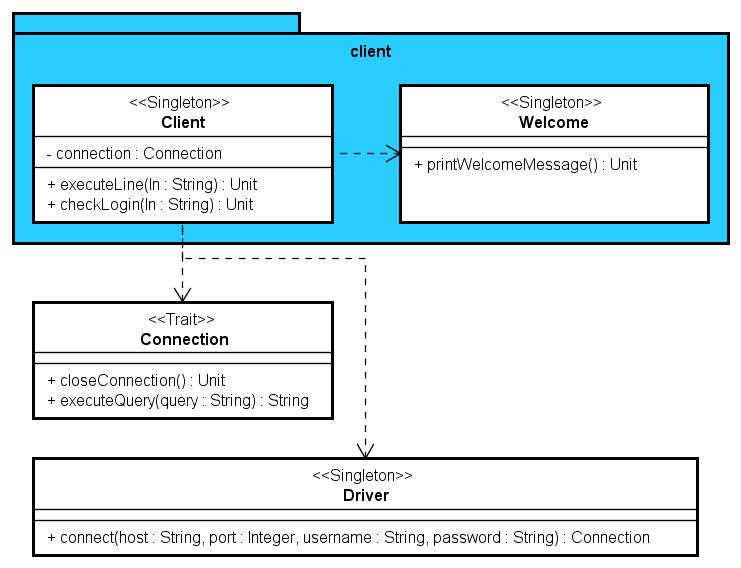
\includegraphics[scale=0.5]{Client/clientLevel.jpg}
			\caption{Componente Actorbase.client}
		\end{figure}
		La componente client di \emph{Actorbase} è un semplice client da riga di comando per interagire con il server attraverso il driver, è composta dalle classi Client e Welcome.
	
	\subsection{Actorbase.client.Client}	
		\textbf{Descrizione}
			\\ \\
			Classe che rappresenta il client a riga di comando di \emph{Actorbase}.
			\\ \\
		\textbf{Utilizzo}
			\\ \\
			Questa classe viene utilizzata per inviare le stringhe inserite dall'utente al driver di \emph{Actorbase} e per visualizzare le risposte del server.
			\\ \\
		\textbf{Classi ereditate}
			\\ \\
			Nessuna.
			\\ \\
		\textbf{Ereditata da}
			\\ \\
			Nessuna.
			\\ \\
		\textbf{Attributi}
			\begin{itemize}
				\item \texttt{private val connection: Connection } - attributo di tipo Connection, definito nel driver, che rappresenta la connessione con il server. Inizialmente nullo, la connessione viene fornita dal driver dopo aver eseguito l'accesso al server correttamente.
			\end{itemize}
			\textbf{Metodo: }\texttt{def main(args: Array[String])}
			\\ \\
			Metodo main del client che avvia il programma. All'avvio stampa il messaggio di benvenuto della classe Welcome, poi rimane in attesa di input da parte dell'utente.
			\\ \\
			Lista parametri del metodo:
			\begin{itemize}
				\item \texttt{args: Array[String] } - Parametro standard del metodo main di \emph{Scala}.
			\end{itemize}
			\textbf{Metodo: }\texttt{def executeLine(ln: String)}
			\\ \\
			Metodo executeLine del client che ha il compito di inviare al driver le stringhe inserite dall'utente tramite l'omonimo metodo della connection. Deve poter riconoscere la stringa di disconnessione, che chiama un metodo diverso della connection, e la stringa di chiusura, che termina il programma. Inoltre è necessario che le altre stringhe siano processate solo se esiste una connessione con il server.
			\\ \\
			Lista parametri del metodo:
			\begin{itemize}
				\item \texttt{ln: String } - Stringa fornita in input dall'utente.
			\end{itemize}
			\textbf{Metodo: }\texttt{def checkLogin(ln:String)}
			\\ \\
			Metodo checkLogin che riconosce tramite un'espressione regolare il comando di connessione. Una volta riconosciuto il comando di connessione chiama il metodo connect del Driver per ottenere una Connection nel caso in cui i dati siano corretti.
			\\ \\
			Lista parametri del metodo:
			\begin{itemize}
				\item \texttt{ln: String } - Stringa fornita in input dall'utente.
			\end{itemize}
			
	\subsection{Actorbase.client.Welcome}	
		\textbf{Descrizione}
			\\ \\
			Classe che stampa un messaggio di benvenuto sulla console del client e alcuni dati riguardanti la macchina che si sta utilizzando.
			\\ \\
		\textbf{Utilizzo}
			\\ \\
			Stampa di un messaggio di benvenuto per l'utente.
			\\ \\
		\textbf{Classi ereditate}
			\\ \\
			Nessuna.
			\\ \\
		\textbf{Ereditata da}
			\\ \\
			Nessuna.
			\\ \\
		\textbf{Attributi}
			\\ \\
			Nessuno.
			\\ \\
			\textbf{Metodo: }\texttt{def printWelcomeMessage(): Unit}
			\\ \\
			Stampa una stringa di benvenuto con il nome del prodotto e la dichiarazione di essere open-source. Inoltre recupera e stampa il nome e la versione del sistema operativo dell'utente, il nome dell'utente e la versione della JVM installata nella macchina dell'utente.
			\\ \\
			Lista parametri del metodo:
			\\ \\
				Nessuno.
			\\ \\
			
	\subsection{Actorbase.driver}
		\begin{figure}[H]
			\centering
			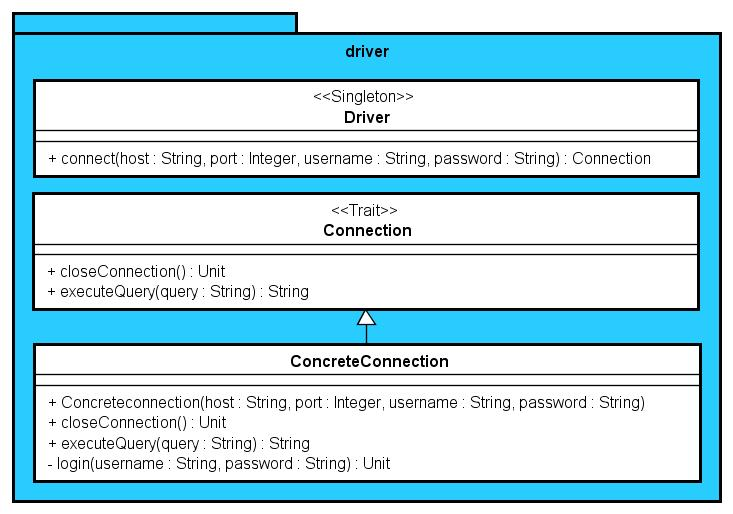
\includegraphics[scale=0.5]{Driver/driverLevel.jpg}
			\caption{Componente Actorbase.driver}
		\end{figure}
		La componente driver di \emph{Actorbase} è un semplice driver per gestire le comunicazioni con il server. \'E composta dalle classi Driver, Connection e ConcreteConnection.
		
	\subsection{Actorbase.driver.Connection (trait)}	
		\textbf{Descrizione}
			\\ \\
			Interfaccia che definisce una connessione con il server di \emph{Actorbase}.
			\\ \\
		\textbf{Utilizzo}
			\\ \\
			Questa interfaccia espone i metodi che deve implementare una classe la concretizza.
			\\ \\
		\textbf{Classi ereditate}
			\\ \\
			Nessuna.
			\\ \\
		\textbf{Ereditata da}
			\begin{itemize}
				\item \texttt{Actorbase.driver.ConcreteConnection}
			\end{itemize}
		\textbf{Attributi}
			\\ \\
			Nessuno.
			\\ \\
			\textbf{Metodo: }\texttt{def closeConnection(): Unit}
			\\ \\
			Metodo astratto per chiudere la connessione con il server.
			\\ \\
			Lista parametri del metodo:
			\\ \\
			Nessuno.
			\\ \\
			\textbf{Metodo: }\texttt{def executeQuery(query: String): String}
			\\ \\
			Metodo astratto per inviare una stringa al server. Ritorna una stringa che rappresenta la risposta del server.
			\\ \\
			Lista parametri del metodo:
			\begin{itemize}
				\item \texttt{query: String } - Stringa da inviare al server.
			\end{itemize}
			
			
	\subsection{Actorbase.driver.ConcreteConnection}	
		\textbf{Descrizione}
			\\ \\
			Concretizzazione della classe Connection.
			\\ \\
		\textbf{Utilizzo}
			\\ \\
			Questa classe riceve delle stringhe tramite il metodo executeLine. Queste stringhe vengono modificate ed inviate al Server. La classe ritorna le risposte alle query in formato di stringa.
			\\ \\
		\textbf{Classi ereditate}
			\begin{itemize}
				\item \texttt{Actorbase.driver.Connection}
			\end{itemize}
		\textbf{Ereditata da}
			\\ \\
			Nessuna.
			\\ \\
		\textbf{Attributi}
			\begin{itemize}
				\item \texttt{private val socket: Socket} - Socket di java.net usato per la connessione con il server.
				\item \texttt{private val out: PrintStream} - PrintStream di java.io usato per scrivere sul socket.
				\item \texttt{private val in: InputStream} - InputStream di java.io usato per leggere dal socket.
				\item \texttt{val host: String} - Nome dell'host.
				\item \texttt{val port: Integer} - Numero della porta su cui impostare la connessione.
				\item \texttt{val username: String} - Nome utente per effettuare il login al server.
				\item \texttt{val password: String} - Password dell'utente per effettuare il login al server.
			\end{itemize}
			\textbf{Costruttore: }\texttt{ConcreteConnection(val host: String, val port: Integer, val username: String, val password: String)}
			\\ \\
			Costruisce un oggetto di tipo Concrete connection.
			\\ \\
			Lista parametri del metodo:
			\begin{itemize}
				\item \texttt{host: String} - Nome dell'host.
				\item \texttt{port: Integer} - Numero della porta su cui impostare la connessione.
				\item \texttt{username: String} - Nome utente per effettuare il login al server.
				\item \texttt{password: String} - Password dell'utente per effettuare il login al server.
			\end{itemize}
			\textbf{Metodo: }\texttt{def closeConnection(): Unit}
			\\ \\
			Chiude la connessione con il server chiudendo il socket e tutti gli stream su di esso.
			\\ \\
			Lista parametri del metodo:
			\\ \\
			Nessuno.
			\\ \\
			\textbf{Metodo: }\texttt{def executeQuery(query: String): String}
			\\ \\
			Prepara la stringa per essere inviata al server, aggiungendo i byte per il protocollo e per l'identificazione della richiesta. Dopo aver inviato la richiesta al server resta in attesa di una risposta per un tempo determinato.
			\\ \\
			Lista parametri del metodo:
			\begin{itemize}
				\item \texttt{query: String} - Query da inviare al server.
			\end{itemize}
			\textbf{Metodo: }\texttt{private def login(username: String, password: String): Unit}
			\\ \\
			Questo metodo deve essere eseguito alla costruzione della classe. Il metodo prova a connettersi al server mandando il comando di login e attende una risposta. In caso di risposta negativa chiude la connessione.
			\\ \\
			Lista parametri del metodo:
			\begin{itemize}
				\item \texttt{username: String} - Nome utente per autenticarsi nel server.
				\item \texttt{password: String} - Password dell'utente per autenticarsi nel server.
			\end{itemize}
			
	\subsection{Actorbase.driver.Driver}	
		\textbf{Descrizione}
			\\ \\
			Driver di \emph{Actorbase}.
			\\ \\
		\textbf{Utilizzo}
			\\ \\
			La classe Driver crea un oggetto di tipo Connection e lo restituisce.
			\\ \\
		\textbf{Classi ereditate}
			\\ \\
			Nessuna.
			\\ \\
		\textbf{Ereditata da}
			\\ \\
			Nessuna.
			\\ \\
		\textbf{Attributi}
			\\ \\
			Nessuno.
			\\ \\
		\textbf{Metodo: }\texttt{def connect(host: String, port: Integer, username: String, password: String): Connection}
			\\ \\
			Questo metodo crea un oggetto di tipo Connection con i parametri passati e lo ritorna al chiamante. Se la connessione non è stata effettuata il metodo ritorna il valore nullo.
			Il metodo deve anche gestire le eccezioni InterruptedException ed Exception.
			\\ \\
			Lista parametri del metodo:
			\begin{itemize}
				\item \texttt{host: String } - Nome dell'host da connettere al server.
				\item \texttt{port: Integer } - Porta sulla quale aprire la connessione.
				\item \texttt{username: String } - Nome dell'utente che vuole accedere al sistema.
				\item \texttt{password: String } - Password dell'utente che vuole accedere al sistema.
			\end{itemize}
			
	\newpage
	
	\section{Diagrammi di sequenza}
	
	\newpage
	
	\section{Tracciamento}
	
	\subsection{Tracciamento requisiti-classi}
	
	\subsection{Tracciamento classi-requisiti}
	
	\subsection{Tracciamento classi-test}

		
	\newpage 
	
	\cleardoublepage
	\addcontentsline{toc}{section}{\listfigurename}
	\listoffigures
	
	\cleardoublepage
	\addcontentsline{toc}{section}{\listtablename}
	\listoftables
		
\end{document}